%Khwopa college of Engineering Latex Template
%Prepared by Mukesh Kumar Pokharel for Project Proposal as references.
\usepackage{tocloft}
% Increase the second argument (the label width) so numbers like "2.1.10" fit cleanly
\documentclass[12pt, a4paper, oneside, openany]{report}

% ── Encoding ──────────────────────────────────────────────────────────────────
\usepackage[utf8]{inputenc}

% ── Page Layout ───────────────────────────────────────────────────────────────
\usepackage[left=1.2in, right=1in, top=1.2in, bottom=1in, 
            headheight=6pt, a4paper]{geometry}

% ── Graphics & Figures ────────────────────────────────────────────────────────
\usepackage{graphicx}
\usepackage{subcaption}
\usepackage{float}

% ── Math ──────────────────────────────────────────────────────────────────────
\usepackage{amsmath, amssymb, amsfonts}
\usepackage{setspace}

% ── Tables ────────────────────────────────────────────────────────────────────
\usepackage{array}
\usepackage{longtable}

% ── Text & Formatting ─────────────────────────────────────────────────────────
\usepackage{ragged2e}
\usepackage{lipsum}
\usepackage{emptypage}
\let\cleardoublepage\clearpage 
\usepackage{placeins}
\setlength{\parskip}{0pt}
\renewcommand{\baselinestretch}{1.5}
\raggedbottom
\usepackage{cleveref}

% ── Bibliography ──────────────────────────────────────────────────────────────
\usepackage{cite}

% ── Section Title Formatting ──────────────────────────────────────────────────
\usepackage{titlesec}

\titleformat{\chapter}[display]
    {\centering\normalfont\large\bfseries}
    {\MakeUppercase{\chaptertitlename} \thechapter}{2pt}{\Large}
\titlespacing{\chapter}{0pt}{0pt}{4pt}

\titleformat{\section}
    {\normalfont\large\bfseries}{\thesection}{1em}{}

\titleformat{\subsection}
    {\normalfont\normalsize\bfseries}{\thesubsection}{1em}{}

\titleformat{\subsubsection}
    {\normalfont\normalsize\bfseries}{\thesubsubsection}{1em}{}

% ── TOC Depth ─────────────────────────────────────────────────────────────────
\setcounter{tocdepth}{3}
\setcounter{secnumdepth}{3}

% ── Hyperref LAST — removes red boxes, enables clickable TOC ──────────────────
\usepackage{hyperref}
\hypersetup{
    colorlinks=false,
    pdfborder={0 0 0},
    linkbordercolor={0 0 0},
    citebordercolor={0 0 0},
    urlbordercolor={0 0 0}
}

% ══════════════════════════════════════════════════════════════════════════════
\begin{document}
\noindent
\let\cleardoublepage\clearpage

    % ── Front Matter ──────────────────────────────────────────────────────────
    \thispagestyle{empty}
\singlespacing
 \begin{center}
		\thispagestyle{empty}
		\Large\textbf{TRIBHUVAN UNIVERSITY}\\
		\Large\textbf{INSTITUTE OF ENGINEERING }\\
		\vspace{0.2in}
		\large{\textbf{Khwopa College Of Engineering}\\}
		\normalsize{Libali, Bhaktapur\\}
		\large\textbf{Department of Computer and Electronics Engineering}
		\vspace{0.2in}
		\begin{figure}[h]
		    \centering
			    
\includegraphics[width=0.25\textwidth]{img/Khwopalogo.jpg}
		\end{figure}
		
		\vspace{0.2in}
		\large{A FINAL REPORT ON\\\textbf{MorphAI:
    Predicting Facial Appearance Transformation\\
    Using Generative Deep Learning}\\}
		
		\vspace{0.2in}
		\large{\textit{Submitted in partial fulfillment of the requirements for the degree in Bachelor of Computer Engineering\\}}
		
		
		%\large{\textbf{BACHELOR OF COMPUTER ENGINEERING}\\}
		
		\vspace{0.2in}
		\large{Submitted by}\\
		\begin{tabular}{p{3.5in}p{3in}}
        %Write name in alphabetical order
    
       \hspace{0.3cm}Kristi Koju& KCE080BCT010\\
        \hspace{0.3cm}Nishana Budha & KCE080BCT017\\
        \hspace{0.3cm}Aamod Baral & KCE080BCT025\\
        \hspace{0.3cm}Reeshav Khyaju & KCE080BCT028\\
		 \vspace{0.2in}
		\end{tabular}
		%\vspace{1cm}
		\large\textbf{Under the Supervision of}\\[0.1cm]
      \normalsize{Er.Anku Jaiswal}\\
      \normalsize{Assistant Professor}\\
      \normalsize{IoE, Pulchowk Campus}\\
      % \normalsize{Leapfrog Technology}\\[0.4cm]
		%	\vspace{1cm}
			\vspace{2cm}
		\large{\textbf{Khwopa College of Engineering}\\}
			\normalsize{Libali, Bhaktapur\\
			August,2026
		}
    \end{center}
\onehalfspacing
    \newgeometry{top=1in}
\pagenumbering{gobble}
\vspace*{1.3in}
\begin{center}
\large{\textbf{CERTIFICATE OF APPROVAL}}
\end{center}
\vspace{1cm}


\noindent
This is to certify that this minor project work entitled \textbf{``MorphAI: Predicting Facial Appearance Transformation Using Generative Deep Learning''}, submitted by Kristi Koju (KCE080BCT010), Nishana Budha (KCE080BCT017), Aamod Baral (KCE080BCT025) and Reeshav Khyaju (KCE080BCT028), has been examined and accepted as the partial fulfillment of the requirements for the degree of Bachelor of Computer Engineering. The project was carried out under special supervision and within the time frame prescribed by the syllabus.


\vspace{2cm}

\noindent
\begin{minipage}[t]{0.45\textwidth}
\centering
..........................................\\
\textbf{Er. Surendra KC} \\
External Examiner \\
Director of Engineering Infinite Software Services
\end{minipage}
\hfill
\begin{minipage}[t]{0.45\textwidth}
\centering


..........................................\\
\textbf{Er. Anku Jaiswal} \\
Project Supervisor \\
Assistant Professor\\
IoE, Pulchowk Campus \\
\end{minipage}

\vspace{1.5cm}

\vspace{0.5cm}
\begin{center}
..........................................\\
\textbf{Er. Dinesh Gothe}\\
Head of Department\\
Department of Computer and Electronics Engineering\\
Khwopa College of Engineering
\end{center}
\newpage

\pagenumbering{roman}
\addcontentsline{toc}{section}{Copyright}
\begin{center}
    {\Large\bfseries COPYRIGHT\copyright}
\end{center}
\vspace{1em}
\normalsize
\justify
The author has agreed that the library of Khwopa College of Engineering may make this report freely available for inspection. Moreover, the author has agreed that permission for extensive copying of this project report for scholarly purposes may be granted by the supervisor who supervised the project work recorded herein or, in their absence, by the Head of the Department where the project report was completed. It is understood that recognition will be given to the author of the report and to the Department of Computer and Electronics Engineering, KhCE, for any use of the material in this project report. Copying, publication, or any other use of this report for financial gain without the approval of the department and the author's written permission is prohibited. Requests for permission to copy or make any other use of the material in this report, in whole or in part, should be addressed to:

\vspace{1.5cm}
\noindent\textbf{Head of Department} \\
Department of Computer and Electronics Engineering \\
Khwopa College of Engineering (KhCE) \\
Libali-08, Bhaktapur, Nepal
\newpage

\addcontentsline{toc}{section}{Acknowledgement}
\begin{center}
    {\Large\bfseries ACKNOWLEDGEMENT}
\end{center}
\vspace{1.2cm}
\normalsize
\noindent
We would like to express our deepest gratitude to our supervisor of the project, \textbf{Er.Anku Jaiswal}, for her immense support and guidance throughout the course of this project. Her insightful advice, expertise, and unwavering support have been crucial to our work's successful completion. This project would not have been possible without her guidance and mentorship.

\noindent We would also like to extend gratitude to our teachers \textbf{Er.Mukesh Kumar Pokharel} and \textbf{Er.Anish Baral} for their constructive feedback and unwavering support throughout the project. The expertise and analytical recommendations gave us fresh viewpoints, which were crucial for improving our project.

\noindent A special thanks to \textbf{Er.Dinesh Gothe} for his encouragement and assistance. We have been greatly inspired by his encouragement, which has kept us dedicated and focused on the project.

\noindent Furthermore, we are grateful to our institution faculty members, and peers for providing us with the necessary resources, facilities, and a conducive learning environment that greatly contributed to our work.

\noindent Finally, we would like to thank everyone who has directly or indirectly assisted us in initiation of our project.

\vspace{1.5cm}
\begin{tabular}{l@{\hspace{3cm}}l}
Kristi Koju & KCE080BCT010\\
Nishana Budha & KCE080BCT017\\
Aamod Baral & KCE080BCT025\\
Reeshav Khyaju & KCE080BCT028\\
\end{tabular}
\newpage

\addcontentsline{toc}{section}{Abstract}
\begin{center}
    {\Large\bfseries ABSTRACT}
\end{center}
\vspace{1em}
\normalsize
\noindent
% Devanagari is the primary script used for writing the Nepali language and contains complex character structures, conjunct consonants, and vowel modifiers that make handwritten text recognition a challenging task. This project aims to develop a Transformer-based Optical Character Recognition (OCR) system for recognizing handwritten Nepali words and converting them into digital text.The proposed system adopts a TrOCR-inspired architecture that combines a pretrained Vision Transformer (ViT) encoder with a lightweight custom BERT-based Transformer decoder. The ViT encoder extracts contextual visual representations from handwritten word images, while the decoder, designed with a compact Transformer configuration and cross-attention mechanism, generates the corresponding Nepali word sequence in Unicode format. Both components are integrated using HuggingFace's VisionEncoderDecoderModel framework to enable end-to-end handwritten word recognition.Experimental results demonstrate that the proposed model achieves a Character Error Rate (CER) of 5.43\%, a Word Error Rate (WER) of 16.58\%, and an overall accuracy of 83.42\%, indicating its effectiveness in recognizing complex handwritten Nepali text. The developed system provides a promising approach for digitizing handwritten Nepali documents and supports the preservation and accessibility of Nepali written resources.
Facial appearance transformation is an important application of generative deep learning that can support facial reconstruction, image editing, and surgical planning. This project aims to develop \textbf{MorphAI}, a generative deep learning system for predicting facial appearance transformation while preserving the identity and structural characteristics of the input face. The proposed system uses a modified Local-Global Network (LGNet) with facial landmark conditioning to reconstruct masked or modified facial regions. MediaPipe Face Mesh is used to extract facial landmarks, which are converted into heatmaps and combined with the masked facial image to provide structural information to the model. The system uses reconstruction, perceptual, style, adversarial, and identity-preservation losses to improve the quality and consistency of the generated facial images. An interactive application allows users to upload an image, select facial regions, and generate the reconstructed facial appearance. The developed MorphAI system provides a promising approach for realistic and identity-aware facial reconstruction and can support future applications in facial image editing and computer-assisted surgical planning.

\vspace{1em}
\noindent
\textbf{Keywords}: \textit{Facial Appearance Transformation, Facial Reconstruction, Generative Adversarial Network, Generative Deep Learning, Identity Preservation, LGNet, MediaPipe Face Mesh.}


\newpage

\tableofcontents
\newpage

\addcontentsline{toc}{section}{List of tables}
\listoftables
\newpage

\addcontentsline{toc}{section}{List of figures}
\listoffigures
\newpage
\addcontentsline{toc}{section}{List of Symbols and Abbreviation}
\begin{center}
    {\Large\bfseries List of Symbols and Abbreviation}
\end{center}
\vspace{0.5em}
\setstretch{1.2}
\noindent\begin{tabular}{ll}
\hline
\textbf{Abbreviation} & \textbf{Full Form} \\
\hline
AI      & Artificial Intelligence \\
AMP     & Automatic Mixed Precision \\
API     & Application Programming Interface \\
BERT    & Bidirectional Encoder Representations from Transformers \\
BOS     & Beginning of Sequence \\
CNN     & Convolutional Neural Network \\
CUDA    & Compute Unified Device Architecture \\
DL      & Deep Learning \\
EOS     & End of Sequence \\
FID     & Fr\'echet Inception Distance \\
FFN     & Feed-Forward Network \\
GAN     & Generative Adversarial Network \\
GELU    & Gaussian Error Linear Unit \\
GPU     & Graphics Processing Unit \\
IIIT    & International Institute of Information Technology \\
IoU     & Intersection over Union \\
L1      & L1 Reconstruction Loss \\
LaMa    & Large Mask Inpainting \\
LGNet   & Large-mask Guided Network \\
LPIPS   & Learned Perceptual Image Patch Similarity \\
MHA     & Multi-Head Attention \\
ML      & Machine Learning \\
MSE     & Mean Squared Error \\
PSNR    & Peak Signal-to-Noise Ratio \\
RGB     & Red, Green, Blue \\
RMSE    & Root Mean Square Error \\
SSIM    & Structural Similarity Index Measure \\
UI      & User Interface \\
VGG     & Visual Geometry Group \\
\hline
\end{tabular}


    % ── Chapters ──────────────────────────────────────────────────────────────
    \chapter{INTRODUCTION}
        \pagenumbering{arabic}
        \section{Background Introduction}


Facial appearance transformation is an important application of generative deep learning. It can be used for facial image editing, facial reconstruction, and other applications where a modified facial region needs to be generated realistically. Recent advances in deep learning have made it possible to reconstruct missing or masked parts of a face while maintaining the overall appearance and identity of the person.

\noindent A face contains many connected features, such as the eyes, eyebrows, nose, and mouth. When one of these regions is removed or modified, generating a realistic replacement requires the model to understand both the local details of the selected region and its relationship with the rest of the face. Generative models such as Generative Adversarial Networks (GANs), autoencoders, and diffusion models have been widely explored for this type of facial reconstruction and editing. PlasticGAN explored facial changes related to plastic and aesthetic surgery, while Mask-aware Photorealistic Facial Attribute Manipulation used facial masks to control changes in specific facial regions \cite{chandaliya2022plasticgan,sun2021maskaware}.

\noindent Several studies have also explored deep learning methods for facial editing and reconstruction. TransEditor used a Transformer-based GAN for controllable facial editing, while Stitch it in Time used a StyleGAN-based approach for editing real facial videos \cite{xu2022transeditor,tzaban2022stitch}. These studies show that generative models can produce realistic facial changes, but many existing approaches are designed for general facial editing and may require complex processing or high computational resources.

\noindent Facial reconstruction has also been studied for applications related to surgical planning. Fang et al. proposed a deep learning method to predict facial appearance changes from planned changes in facial bone structure \cite{fang2022acmt}. Bini et al. combined image inpainting and depth estimation for facial reconstruction and surgical outcome prediction \cite{bini2025facial}. Similarly, Xu et al. developed a diffusion-based method for restoring facial regions while preserving identity \cite{xu2024diffuse}. These studies show the importance of maintaining facial structure and identity when reconstructing facial images.

\newpage
\noindent Facial landmarks can provide useful structural information for facial reconstruction. DeepFaceReshaping demonstrated the use of facial landmarks to control facial reshaping \cite{chen2024deepface}. In MorphAI, facial landmarks are extracted using MediaPipe Face Mesh and are used to generate a heatmap that provides additional facial structure information to the model. The system supports reconstruction of selected facial regions, including the left eye, right eye, left eyebrow, right eyebrow, nose, and mouth. It also supports different mask sizes for testing the reconstruction process.

\noindent Based on these ideas, this project proposes \textbf{MorphAI: Predicting Facial Appearance Transformation Using Generative Deep Learning}. The system uses a modified Local-Global Network (LGNet) as the generator to reconstruct masked facial regions. The model receives the masked image together with the mask and facial landmark heatmap as input. During training, a PatchGAN-based discriminator is used with the generator to improve the realism of the reconstructed images. The training process uses reconstruction, perceptual, style, identity, and facial landmark losses to guide the generation process.

\noindent The developed MorphAI application allows a user to upload a facial image, select a facial region or mask type, and generate a reconstructed result. The system provides the original image, masked image, and reconstructed image for comparison. It also calculates image quality and identity-related metrics during evaluation.


        \section{Motivation}
Facial appearance reconstruction is challenging because a realistic result must preserve the important features and identity of the input face while generating the missing or masked regions naturally. Existing facial editing and reconstruction methods use different approaches, including GANs, diffusion models, and landmark-based methods, but many are computationally expensive or are designed for general facial editing rather than controlled facial region reconstruction. These limitations motivate the development of a system that can use facial structural information to guide the reconstruction process. MorphAI addresses this problem by combining facial landmarks extracted using MediaPipe Face Mesh with a modified LGNet-based generative model to reconstruct selected facial regions. The use of landmark information, adversarial learning, and identity-related constraints aims to produce realistic facial reconstructions while maintaining the overall appearance of the input face.


        \section{Problem Statement}

Facial appearance reconstruction in MorphAI involves several key challenges:

\begin{itemize}

\item \textbf{Realistic reconstruction:} The missing or masked facial region should look natural and match the surrounding face.

\item \textbf{Identity preservation:} The reconstruction should preserve the important facial characteristics of the original person.

\item \textbf{Facial structure:} Facial features have fixed spatial relationships, so the generated region should be correctly aligned with the rest of the face.

\item \textbf{Different facial regions:} The system needs to reconstruct different regions such as the eyes, eyebrows, nose, and mouth while maintaining a consistent facial appearance.

\item \textbf{Guidance from landmarks:} The masked image alone may not provide enough structural information. Facial landmarks can help the model understand the position and shape of important facial features.

\item \textbf{Realistic image generation:} The generated result should have clear details and appear visually similar to a real face. Adversarial learning helps improve the realism of the reconstructed image.

\item \textbf{Limitations of existing methods:} Many existing facial editing and reconstruction methods require complex processing or high computational resources. MorphAI aims to provide a practical approach using a modified LGNet with facial landmark information and generative learning \cite{xu2024diffuse,xu2022transeditor,tzaban2022stitch}.

\end{itemize}

%         \section{Problem Statement}
% \begin{itemize}
%     \item Handwritten Nepali word recognition is challenging due to the complex Devanagari script, which includes conjunct consonants, vowel modifiers, and variations in individual handwriting styles \cite{baral2019handwritten,ghimire2020nepali}.
%     \item Existing systems based on CNNs or handcrafted features struggle to capture long-range dependencies and sequential context, and the lack of large, diverse Nepali handwriting datasets limits model accuracy and generalization \cite{hasan2023optical,li2023trocr}.
% \end{itemize}

\section{Objective}

The main objective of this project is:

\begin{itemize}
\item To develop \textbf{MorphAI}, a generative deep learning system for predicting facial appearance transformation using facial landmarks to guide reconstruction while preserving the identity and structure of the input face.
\end{itemize}

\clearpage
\subsection*{Scope Clarification: Reconstruction vs. Surgical Prediction}
It is important to clarify the distinction between facial image reconstruction and 
clinical surgical outcome prediction. MorphAI is a deep learning-based facial image 
inpainting and reconstruction framework: it reconstructs synthetically masked facial 
regions (such as the eyes, eyebrows, nose, and mouth) using surrounding facial context 
and landmark-based structural information. The system does not simulate biological 
tissue deformation, healing processes, anatomical changes, or actual post-operative 
surgical outcomes. Since the experiments use the CelebA-HQ dataset with synthetically applied masks rather than real clinical pre-operative and post-operative patient data, MorphAI's output should be interpreted as a facial reconstruction result and not as a prediction of how a person's face would look after surgery.

\section{Scope of Project}
The scope of this project includes:
\begin{itemize}
    \item Developing a generative deep learning system for facial region reconstruction (inpainting) using synthetically masked facial images.
    
    \item Reconstructing selected facial regions such as the eyes, eyebrows, nose, and mouth from a masked facial image using landmark-conditioned generation.
    
    \item Extracting facial landmarks using MediaPipe Face Mesh to provide structural guidance for the reconstruction process.
    
    \item Evaluating reconstruction quality and identity preservation using standard image-quality and face-recognition metrics.
\end{itemize}

\subsection*{Potential Future Applications}
While MorphAI currently focuses on facial region reconstruction, the approach could be 
extended to other areas in the future. These are possible directions, not features that 
have been built or tested:

\begin{itemize}
    \item \textbf{Facial Image Editing and Restoration:} The same reconstruction approach 
    could be used to fix damaged or blocked parts of facial images in general, not just 
    the regions tested in this project.
    
    \item \textbf{CCTV/Video Restoration:} With further work, this method could help 
    reconstruct faces that are partly blocked or hidden in low-quality surveillance footage.
    
    \item \textbf{AR/VR and Gaming:} The landmark-based approach could be adapted for 
    building or completing facial avatars in AR/VR and gaming applications.
    
    \item \textbf{Surgical Visualization:} This could be a starting point for future 
    research into facial visualization tools. However, MorphAI has not been trained or 
    tested on real clinical data, so it is not ready for actual surgical planning or 
    predicting surgical outcomes. That would require real before-and-after patient data 
    and proper clinical testing, which is beyond the scope of this project.
\end{itemize}

    
    
    \chapter{LITERATURE REVIEW}

\section{Literature Review}

\noindent Facial appearance transformation has developed from traditional image editing to deep learning-based methods such as GANs, Transformers, and diffusion models. These methods can reconstruct or modify facial regions, but maintaining the person's identity and natural facial structure is still challenging.

\noindent GAN-based methods such as PlasticGAN and mask-aware facial manipulation have shown good results in facial editing \cite{chandaliya2022plasticgan,sun2021maskaware}. Other methods, including TransEditor and Stitch it in Time, have improved controllable facial editing \cite{xu2022transeditor,tzaban2022stitch}. However, many existing methods require high computational resources or are designed mainly for general facial editing.

\noindent Recent studies have also explored facial reconstruction for surgical planning and appearance prediction \cite{fang2022acmt,bini2025facial}. Diffusion and landmark-based methods have further improved facial restoration and structural control \cite{xu2024diffuse,chen2024deepface}. These studies provide the basis for MorphAI, which uses MediaPipe Face Mesh landmarks and a modified LGNet to reconstruct selected facial regions while preserving facial structure and identity.



\subsection{Diffuse and Restore: A Region-Adaptive Diffusion Model for Identity-Preserving Blind Face Restoration (2024)}

Xu et al. (2024) proposed a diffusion-based method for restoring degraded facial images while preserving identity. The model uses an Identity Preserving Conditioner (IPC) with a Conditional Diffusion Probabilistic Model (DDPM) to restore facial regions. However, it focuses mainly on face restoration rather than facial appearance transformation or surgical prediction \cite{xu2024diffuse}.

\subsection{PlasticGAN: Holistic Generative Adversarial Network on Face Plastic and Aesthetic Surgery (2022)}

Chandaliya and Nain (2022) proposed PlasticGAN for generating facial appearance changes related to plastic and aesthetic surgery. The model uses a GAN with age and gender information to generate realistic facial transformations. However, the study uses relatively low-resolution images and a limited evaluation setup \cite{chandaliya2022plasticgan}.

\subsection{TransEditor: Transformer-Based Dual-Space GAN for Highly Controllable Facial Editing (2022)}

Xu et al. (2022) introduced TransEditor, which combines a Transformer with StyleGAN2 to provide controlled facial editing. It separates facial structure and appearance into different latent spaces to achieve realistic modifications. However, the method requires latent inversion and considerable computational resources \cite{xu2022transeditor}.

\subsection{Stitch it in Time: GAN-Based Facial Editing of Real Videos (2022)}

Tzaban et al. (2022) proposed a StyleGAN2-based method for editing facial attributes in real videos while maintaining identity and temporal consistency. The method produces smooth facial changes without noticeable flickering. However, it is mainly designed for video editing rather than facial reconstruction or surgical appearance prediction \cite{tzaban2022stitch}.

\subsection{Deep Learning Framework for Facial Reconstruction Outcome Prediction (2025)}

Bini et al. (2025) proposed a deep learning framework for facial reconstruction and computer-assisted surgical planning. The study combines image inpainting and depth estimation and evaluates different models for facial reconstruction. However, the approach does not specifically focus on identity preservation, which is an important aspect of the proposed MorphAI system \cite{bini2025facial}.


\subsection{DeepFaceReshaping: Interactive Deep Face Reshaping via Landmark Manipulation (2024)}

Chen et al. (2024) proposed an interactive facial reshaping method based on facial landmark manipulation. The framework combines Graph VAE, Conditional GAN, Transformer, and U-Net to generate realistic facial changes. However, it mainly focuses on 2D facial editing and is not specifically designed for surgical outcome prediction \cite{chen2024deepface}.

\clearpage
\subsection{Deep Learning-based Facial Appearance Simulation Driven by Surgically Planned Craniomaxillofacial Bony Movement (2022)}

Fang et al. (2022) proposed a deep learning method for simulating facial appearance changes based on surgically planned craniomaxillofacial bone movement. The approach learns the relationship between structural changes and facial appearance. However, it requires specialized patient-specific anatomical data and focuses mainly on craniomaxillofacial surgical simulation \cite{fang2022acmt}.


\subsection{Mask-aware Photo Facial Attribute Manipulation (2021)}

Sun et al. (2021) proposed a mask-aware method for controlling facial attribute manipulation. The approach uses masked facial regions to guide the generation process while maintaining realistic facial details. However, it focuses on facial attribute editing rather than facial reconstruction for surgical prediction, and additional constraints are needed to preserve identity and facial details \cite{sun2021maskaware}.


\subsection{Research Gap}

Previous studies have shown good results in facial restoration, editing, and surgical appearance prediction. However, most methods focus on general face editing, image restoration, or complex surgical simulation rather than localized facial transformation.
\newline
Another issue is identity preservation. A generated face may look realistic but still change the person's identity or facial structure. Some methods also require large computational resources or special 3D patient data, which may not be practical for a simple image-based system.
\newline
Therefore, there is a need for a simpler framework that can transform a selected facial region while keeping the person's identity and facial structure. MorphAI addresses this gap by combining MediaPipe Face Mesh landmarks with a modified LGNet model and ArcFace-based identity loss. This allows the system to use facial structure as guidance and generate realistic facial reconstruction using only 2D facial images.


\section{Related Theories}
\subsection{Facial Image Reconstruction}

Facial image reconstruction aims to recover missing or corrupted regions of a face using the surrounding information. In MorphAI, this is treated as a guided facial inpainting problem where a mask indicates the region to be reconstructed.

\noindent The masked image is obtained as:

\begin{equation}
I_{\text{masked}} = I \odot (1-M)
\end{equation}

\noindent where $I$ is the original image, $M$ is the binary mask, and $\odot$ denotes element-wise multiplication.

\subsection{Facial Landmark Detection}

Facial landmark detection identifies important points such as the eyes, eyebrows, nose, and mouth. MorphAI uses these points to provide facial structure information and to generate semantic masks and landmark heatmaps.

\subsection{MediaPipe Face Mesh}

MediaPipe Face Mesh is used in MorphAI to extract facial landmarks from input images. The detected landmarks are grouped into facial regions and used for mask generation and structural guidance.

\subsection{Facial Region Masking}

Facial masking identifies the region that needs to be reconstructed. MorphAI uses both semantic facial masks and random rectangular masks. Semantic masks are generated from facial landmarks and can represent regions such as the eyes, eyebrows, nose, and mouth.

\subsection{Generative Adversarial Networks}

Generative Adversarial Networks (GANs) consist of a generator and a discriminator. The generator produces reconstructed images, while the discriminator evaluates whether the generated results appear realistic.

\noindent In MorphAI, adversarial learning helps improve the visual quality and realism of reconstructed facial regions.

\subsection{Generator and Discriminator}

The generator reconstructs the masked facial region using the available image information, mask, and landmark guidance. The discriminator evaluates the generated image against real facial images.

\noindent Together, they encourage the generator to produce realistic facial details and textures.

\subsection{PatchGAN}

PatchGAN evaluates local image patches instead of judging the complete image with a single value. This allows the discriminator to focus on details such as skin texture, eyes, lips, and facial boundaries.

\noindent MorphAI uses a PatchGAN discriminator to improve the local realism of reconstructed facial regions.

\subsection{Local-Global Network (LGNet)}

LGNet uses local and global information to reconstruct missing image regions. The local pathway focuses on details inside the missing region, while the global pathway uses surrounding information to maintain overall consistency.

\noindent MorphAI uses a modified LGNet generator with landmark heatmap guidance. The generator receives the masked image, facial mask, and landmark heatmap:

\begin{equation}
\hat{I}_{\text{raw}}
=
G(I_{\text{masked}},M,H)
\end{equation}

where $G$ represents the LGNet generator and $H$ represents the landmark heatmap.

\subsection{Loss Functions}

MorphAI uses multiple loss components to guide facial reconstruction and
preserve visual quality, texture, identity, and facial structure. The main
loss components are:

\begin{itemize}

    \item \textbf{L1 Loss:} Measures the pixel-level difference between the
    reconstructed image and the target image. It helps the model produce
    accurate pixel-level reconstruction.

    \begin{equation}
    \mathcal{L}_{L1} =
    \frac{1}{CHW}
    \sum_{c,h,w}
    \left|
    \hat{I}_{c,h,w} - I_{c,h,w}
    \right|
    \end{equation}

    \item \textbf{Perceptual Loss:} Compares deep feature representations
    of the reconstructed and target images. It helps preserve important
    facial structures and visual details.

    \begin{equation}
    \mathcal{L}_{perceptual} =
    \sum_j
    \frac{1}{C_jH_jW_j}
    \left|
    \phi_j(\hat{I})-\phi_j(I)
    \right|_1
    \end{equation}

    \item \textbf{Style Loss:} Compares feature correlations between the
    reconstructed and target images to maintain similar texture and
    appearance.

    \begin{equation}
    \mathcal{L}_{style} =
    \sum_j
    \frac{1}{C_j^2}
    \left|
    G_j(\hat{I})-G_j(I)
    \right|_1
    \end{equation}

    \item \textbf{Identity Loss:} Encourages the reconstructed face to
    preserve the identity of the input subject using facial feature
    embeddings and cosine similarity.

    \begin{equation}
    \mathcal{L}_{identity} =
    1-
    \frac{
    f(\hat{I})\cdot f(I)
    }{
    \|f(\hat{I})\|_2\|f(I)\|_2
    }
    \end{equation}

    \item \textbf{Facial Landmark Loss:} Encourages the reconstructed
    image to maintain the correct position of important facial features.

    \begin{equation}
    \mathcal{L}_{landmark} =
    \frac{1}{N}
    \sum_{k=1}^{N}
    \operatorname{Wing}
    \left(
    \operatorname{Det}(\hat{I})_k-
    \operatorname{Det}(I)_k
    \right)
    \end{equation}

    \item \textbf{Adversarial Loss:} Encourages the generator to produce
reconstructions that the PatchGAN discriminator cannot distinguish from
real facial images, improving perceptual realism and local texture detail.

% % --- if your discriminator uses BCE (vanilla GAN) ---
% \begin{equation}
% \mathcal{L}_{\text{adv}} = \mathbb{E}_{I}\left[\log D(I)\right] +
% \mathbb{E}_{\hat{I}}\left[\log(1 - D(\hat{I}))\right]
% \label{eq:adv-loss}
% \end{equation}

% --- OR if your discriminator uses MSE (LSGAN, more typical for PatchGAN) ---
\begin{equation}
\mathcal{L}_{\text{adv}} = \mathbb{E}_{I}\left[(D(I) - 1)^2\right] +
\mathbb{E}_{\hat{I}}\left[D(\hat{I})^2\right]
\label{eq:adv-loss}
\end{equation}

where $D$ denotes the PatchGAN discriminator, $I$ the ground-truth facial
image, and $\hat{I}$ the reconstructed image generated by LGNet.

\end{itemize}

\subsection{Identity Preservation}

Identity preservation ensures that the reconstructed face remains visually
consistent with the input subject. MorphAI uses facial embeddings and
ArcFace-based similarity during evaluation to measure identity preservation.

\subsection{Boundary Blending and Post-processing}
The reconstructed region may contain visible boundaries between the generated
and original areas. MorphAI therefore applies blending during post-processing
to create a smoother transition between the reconstructed region and the
surrounding face.
\noindent For alpha feathering:
\begin{equation}
\alpha = M * G_{\sigma}
\end{equation}
\noindent where $G_{\sigma}$ represents a Gaussian kernel. The final blended image is
given by:
\begin{equation}
I_{\text{final}}
=
\alpha\hat{I}
+
(1-\alpha)I_{\text{bg}}
\end{equation}
\noindent where $\hat{I}$ is the reconstructed image and $I_{\text{bg}}$ is the original
background.

\noindent In addition to alpha feathering, MorphAI also supports \textbf{seamless 
Poisson cloning} as a blending option. Instead of blending pixel values directly, 
Poisson blending matches the gradients of the reconstructed region to the 
surrounding image, producing smoother colour and illumination consistency across 
the boundary at a higher computational cost than alpha feathering. Both options 
are available to the user in the MorphAI interface, allowing a trade-off between 
blending speed and visual smoothness.

\subsection{Evaluation Metrics}

MorphAI evaluates facial reconstruction using pixel-level, structural,
perceptual, realism, and identity-based metrics:

\begin{itemize}

\item \textbf{Peak Signal-to-Noise Ratio (PSNR):} Measures pixel-level
similarity between the reconstructed and target images. Higher values
indicate better reconstruction quality.

\item \textbf{Structural Similarity Index Measure (SSIM):} Measures
structural similarity between the reconstructed and target images.
Higher values indicate better preservation of facial structure.

\item \textbf{Learned Perceptual Image Patch Similarity (LPIPS):}
Measures perceptual similarity using deep image features. Lower values
indicate greater perceptual similarity.

\item \textbf{Fréchet Inception Distance (FID):} Compares the feature
distributions of reconstructed and real images. Lower values generally
indicate better visual realism.

\item \textbf{Identity Similarity:} Measures how well the reconstructed
face preserves the identity of the input subject using facial embeddings
and cosine similarity. Higher values indicate better identity
preservation. ArcFace is used for identity evaluation.

\item \textbf{Root Mean Square Error (RMSE):} Measures the pixel-level
reconstruction error between the reconstructed and target images.
Lower values indicate smaller reconstruction errors.

\item \textbf{RMSE-log:} Measures reconstruction error after applying a
logarithmic transformation to the reconstructed and ground-truth images,
reducing the influence of large pixel differences. Lower values indicate
smaller reconstruction errors. The full mathematical formulation is given
in Section~\ref{sec:rmse-log} (Eq.~\ref{eq:rmse-log}).

\end{itemize}



\subsection{Dataset}

\subsubsection{Dataset Description}

MorphAI uses the CelebA-HQ dataset for facial image reconstruction. The
dataset contains high-quality facial images with diverse identities,
expressions, poses, and appearances. The images are used as ground-truth
facial images for training and evaluation.

\noindent During training, facial regions are artificially masked so that
the model learns to reconstruct the missing areas. The images are resized
to $256 \times 256$ pixels to match the input requirements of the LGNet
generator.

\noindent It is important to note that CelebA-HQ contains only single, unpaired facial images -- 
it does not provide real before-and-after surgical image pairs. The facial reconstruction 
task used to train and evaluate MorphAI is created artificially: selected facial regions 
are synthetically masked on an otherwise complete image, and the original unmasked image 
serves as the ground truth for reconstruction. No real pre-operative or post-operative 
surgical patient dataset is used anywhere in this project. This synthetic masking 
approach approximates a region-completion task; it does not model or represent actual 
surgical tissue change.

\subsubsection{Dataset Preprocessing}

The facial images are resized to $256 \times 256$ pixels and processed
before being provided to the model. Facial landmarks are extracted using
MediaPipe Face Mesh and are used to provide structural information about
the face.

\noindent The RGB image, binary facial mask, and landmark heatmap are
combined to form a five-channel input:

\begin{equation}
3\text{ RGB channels} + 1\text{ mask channel} + 1\text{ heatmap channel}
= 5\text{ channels}.
\end{equation}

\noindent Therefore, the input to the LGNet generator has the dimensions
$5 \times 256 \times 256$.

\subsubsection{Dataset Split}

The CelebA-HQ dataset is divided into training, validation, and test sets.
The training set is used to optimize the model, the validation set is used
to monitor training performance, and the test set is used for final
evaluation.

\subsubsection{Mask Generation}

MorphAI uses facial region masks to simulate missing parts of the face.
The masks are generated for different facial regions, including:

\begin{itemize}
    \item \textbf{Eyes and eyebrows}
    \item \textbf{Nose}
    \item \textbf{Mouth}
\end{itemize}

\noindent These masks allow the model to learn how to reconstruct different
parts of the face from the available surrounding information.

\subsubsection{Data Representation}

Each training sample consists of an RGB facial image, a binary mask, and a
landmark heatmap. These components are combined as:

\begin{equation}
X = [I_{\text{RGB}}, M, H]
\end{equation}

\noindent where $I_{\text{RGB}}$ represents the facial image, $M$ represents
the facial mask, and $H$ represents the landmark heatmap.


\subsubsection{Dataset Challenges}

The main challenges associated with using CelebA for MorphAI include:

\begin{itemize}
    \item \textbf{Initially:} During facial alignment of the CelebA
    images, inaccurate landmark detection occasionally caused improper
    alignment and cropping, particularly around the chin region.
    
    \item \textbf{Image Alignment:} Facial images require proper alignment
    to maintain consistent facial structure and improve the reconstruction
    process.

    \item \textbf{Image Resizing:} Images must be resized to the required
    $256 \times 256$ resolution while preserving important facial details.

    

    \item \textbf{Synthetic Masking:} The dataset does not provide actual
    before-and-after facial surgery pairs, so missing regions are created
    artificially.

    \item \textbf{Facial Variation:} Differences in pose, expression, and
    appearance can make facial reconstruction more challenging.

    \item \textbf{Lighting Variation:} Changes in illumination may affect
    the appearance and reconstruction of facial regions.

    \item \textbf{Landmark Accuracy:} Incorrect facial landmarks can affect
    the generated landmark heatmap and reconstruction quality.

\end{itemize}



% \newpage
\section{Review Matrix}

\setlength{\LTpre}{0pt}
\setlength{\LTpost}{0pt}
\renewcommand{\arraystretch}{1.3}
\noindent Table~\ref{tab:review-matrix} presents a summary of the literature reviewed for the MorphAI project, highlighting key methodologies, datasets, and limitations in facial appearance transformation and reconstruction.


% \noindent Table~\ref{tab:review-matrix} presents a summary of the literature reviewed in this chapter. It consolidates key studies, their methodologies, and contributions, providing a clear overview of the evolution of handwritten text recognition techniques.




\begin{longtable}[l]{|c|p{3.2cm}|p{3.2cm}|p{2.5cm}|p{4.0cm}|}

\caption{Summary of Reviewed Literature for MorphAI}
\label{tab:review-matrix} \\

\hline

\textbf{S.N.} &
\textbf{Author(s) \& Year} &
\textbf{Method} &
\textbf{Dataset} &
\textbf{Limitations} \\ \hline

\endfirsthead

\multicolumn{5}{c}%
{\textbf{Table \thetable\ (continued)}} \\ \hline

\textbf{S.N.} &
\textbf{Author(s) \& Year} &
\textbf{Method} &
\textbf{Dataset} &
\textbf{Limitations} \\ \hline

\endhead

\hline
\multicolumn{5}{r}{\textit{Continued on next page}} \\
\endfoot

\hline
\endlastfoot

1 &
Xu et al. (2024) \cite{xu2024diffuse} \newline
\textit{Diffuse and Restore} &
Identity Preserving Conditioner (IPC) + Conditional DDPM &
FFHQ, CelebA-Test &
Designed for face restoration rather than surgical prediction; diffusion-based models require high computational resources. \\ \hline

2 &
Chandaliya and Nain (2022) \cite{chandaliya2022plasticgan} \newline
\textit{PlasticGAN: Holistic Generative Adversarial Network on Face Plastic and Aesthetic Surgery} &
GAN with age and gender conditioning &
CACD, UTKFace, CLF, Adience &
Uses a small evaluation dataset and relatively low image resolution ($128\times128$); based on an older GAN architecture. \\ \hline

3 &
Xu et al. (2022) \cite{xu2022transeditor} \newline
\textit{TransEditor} &
StyleGAN2 + Transformer + Dual Latent Space &
FFHQ, CelebA-HQ &
Requires latent inversion and high GPU memory; performance can be affected by large pose variations. \\ \hline

4 &
Tzaban et al. (2022) \cite{tzaban2022stitch} \newline
\textit{Stitch it in Time} &
StyleGAN2-based GAN &
FFHQ &
Designed primarily for facial video editing rather than surgical prediction and requires considerable computational resources. \\ \hline

5 &
Bini et al. (2025) \cite{bini2025facial} \newline
\textit{AI-Based Facial Reconstruction for Surgical Outcome Prediction} &
LGNet + DepthPro &
FFHQ, C3I-SynFace &
Uses benchmark datasets instead of real patient data; healing processes and tissue deformation are not modeled. \\ \hline

6 &
Chen et al. (2024) \cite{chen2024deepface} \newline
\textit{DeepFaceReshaping} &
Graph VAE + Conditional GAN + Transformer + U-Net &
CelebA-HQ &
Limited to 2D facial editing and mainly frontal faces; not specifically designed for clinical surgical prediction. \\ \hline

7 &
Fang et al. (2022) \cite{fang2022acmt} \newline
\textit{Deep Learning-based Facial Appearance Simulation Driven by Surgically Planned Craniomaxillofacial Bony Movement} &
Attentive Correspondence assisted Movement Transformation Network (ACMT-Net) &
Patient-specific facial and bony structure data &
Focuses on facial appearance prediction driven by surgically planned bony movement; requires specialized anatomical data and is mainly intended for craniomaxillofacial surgical simulation. \\ \hline

8 &
Sun et al. (2021) \cite{sun2021maskaware} \newline
\textit{Mask-aware Photorealistic Facial Attribute Manipulation} &
Mask-Adversarial Autoencoder (M-AAE): VAE + GAN &
Facial attribute manipulation datasets &
Focuses on facial attribute manipulation rather than surgical prediction; additional supervision is required to maintain identity and facial details. \\ \hline

\end{longtable}




    \chapter{METHODOLOGY}    

\section{MorphAI System Workflow Diagram}
      \begin{figure}[H]
        \centering
        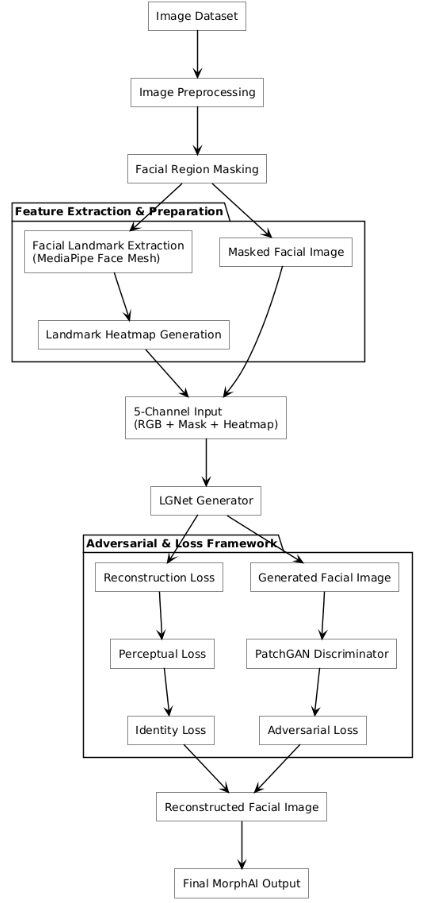
\includegraphics[scale=0.9]{img/model_arch.png}
        \caption{Stages of MorphAI System}
        \label{fig:blockdiagram}
    \end{figure}

\clearpage
\section{Description of Working Flow of the System}

The working process of MorphAI consists of several stages, starting from the input facial image and ending with the reconstructed facial image. The main stages of the system are described below.

\subsection{Image Dataset}

MorphAI uses facial images as the input dataset for training and evaluation. The original facial images are treated as ground-truth images. During training, different facial regions are masked so that the model learns to reconstruct the missing regions.

\subsection{Image Preprocessing}

The input images are resized and converted into a suitable format for the model. Facial landmark detection is then performed on the processed images to obtain the structural information required by the reconstruction system.

\subsection{Facial Region Masking}

A facial region is selected for reconstruction using a binary mask. The mask identifies the area that will be removed or hidden from the input image. MorphAI supports facial regions such as the eyes, eyebrows, nose, and mouth.

\subsection{Feature Extraction and Preparation}

After masking, the system prepares the information required by the reconstruction model. MediaPipe Face Mesh is used to extract facial landmarks from the input image.

\noindent The detected landmarks are then used to generate a landmark heatmap. The heatmap provides additional information about the position and structure of facial features.

\noindent At the same time, the masked facial image is prepared as a separate input. These components are then combined to form the model input.

\clearpage
\subsection{Five-Channel Input Formation}

MorphAI combines the RGB image, facial mask, and landmark heatmap to create a five-channel input:
\begin{equation}
3\text{ RGB channels} + 1\text{ mask channel} + 1\text{ heatmap channel}
= 5\text{ channels}.
\end{equation}

\noindent The resulting input has the form:

\begin{equation}
X \in \mathbb{R}^{5 \times 256 \times 256}.
\end{equation}

\noindent This allows the generator to use both visual information and facial structural information during reconstruction.

\subsection{LGNet Generator}

The five-channel input is passed to the modified LGNet generator. The generator uses the visible facial information, mask, and landmark heatmap to reconstruct the missing facial region.

\noindent The output of the generator is a generated facial image containing the reconstructed region.

\subsubsection{Loss Framework}
The generated image is optimized using a composite loss framework during
training. The loss function combines reconstruction, perceptual, style,
identity, facial landmark, and adversarial losses to guide the generator
toward accurate reconstruction, preservation of facial structure, texture
consistency, identity preservation, and visual realism. The individual
loss terms are defined, and the total
training objective is given by:

\begin{equation}
\mathcal{L}_{\text{total}} = \lambda_{1}\mathcal{L}_{\text{L1}} +
\lambda_{\text{perc}}\mathcal{L}_{\text{perceptual}} +
\lambda_{\text{style}}\mathcal{L}_{\text{style}} +
\lambda_{\text{id}}\mathcal{L}_{\text{identity}} +
\lambda_{\text{lm}}\mathcal{L}_{\text{landmark}} +
\lambda_{\text{adv}}\mathcal{L}_{\text{adv}}
\label{eq:total-loss}
\end{equation}

\noindent where $\lambda_{1}$, $\lambda_{\text{perc}}$, $\lambda_{\text{style}}$,
$\lambda_{\text{id}}$, $\lambda_{\text{lm}}$, and $\lambda_{\text{adv}}$
are the weighting coefficients for each loss term.

\subsection{Reconstructed Facial Image}

After the generator and loss-based optimization, the reconstructed facial image is obtained. The generated region is combined with the remaining facial region to produce a complete reconstructed face.

\clearpage
\subsubsection{Final MorphAI Output}
The final output of MorphAI is the reconstructed facial image. The output is
intended to preserve the facial structure, appearance, and identity of the input
image while reconstructing the selected facial region.

\section{Model Architecture}

% \begin{figure}[H]
%     \centering
%     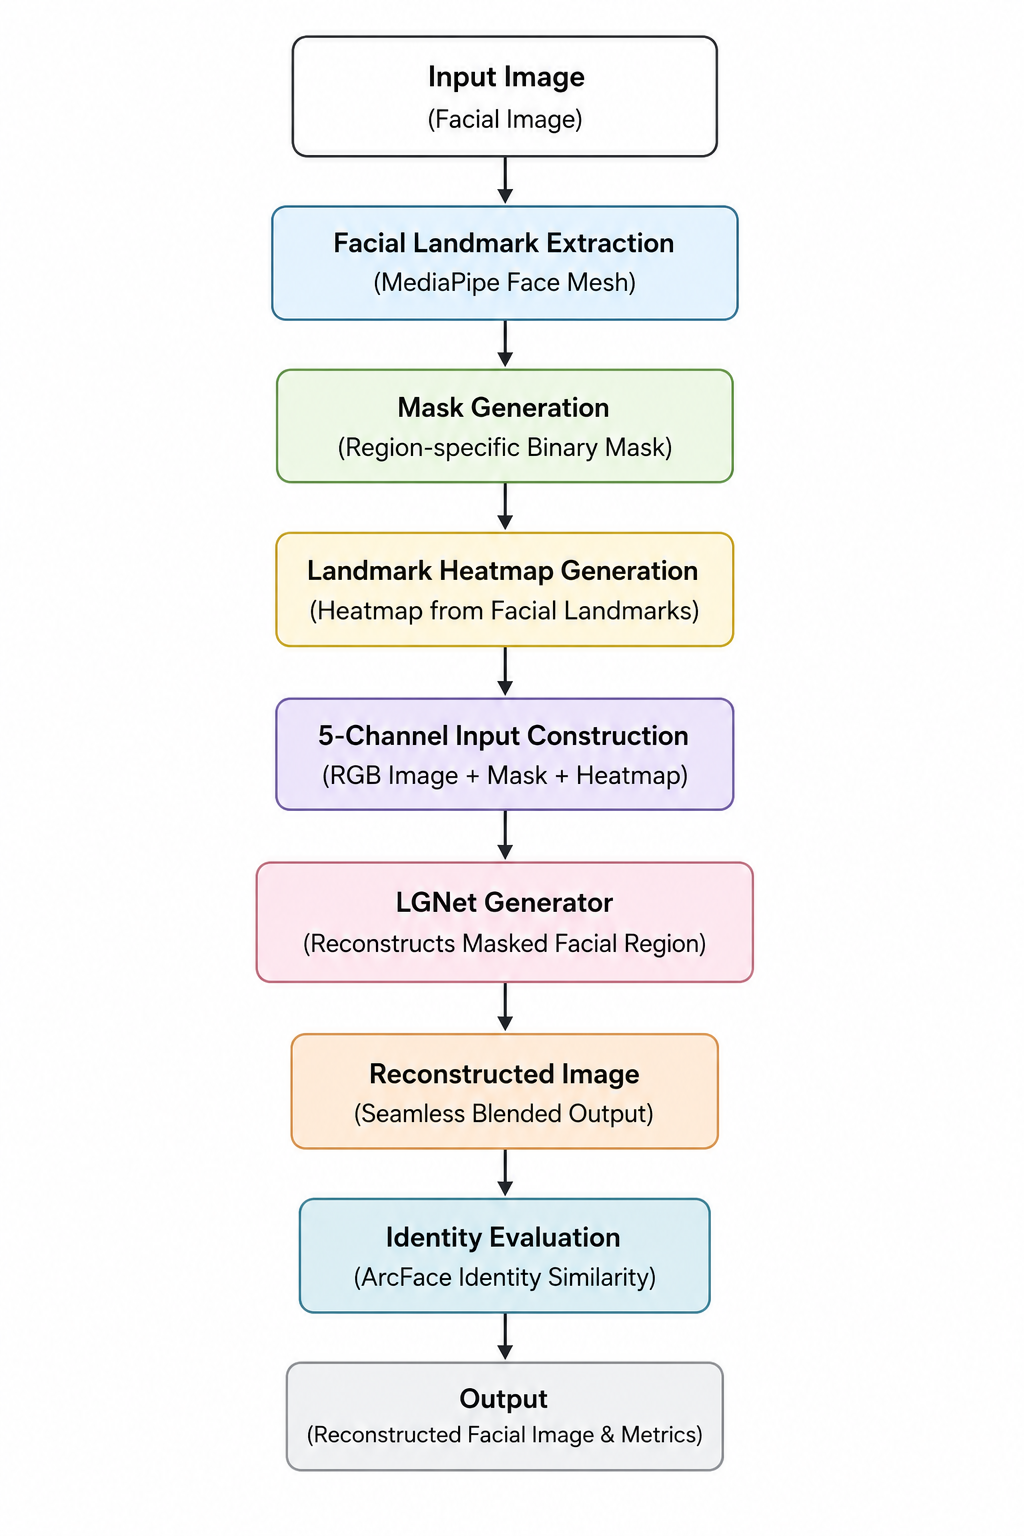
\includegraphics[width=0.85\textwidth]{img/morphai_architecture.png}
%     \caption{MorphAI model architecture}
%     \label{fig:morphai_architecture}
% \end{figure}

\begin{figure}[htbp]
    \centering
    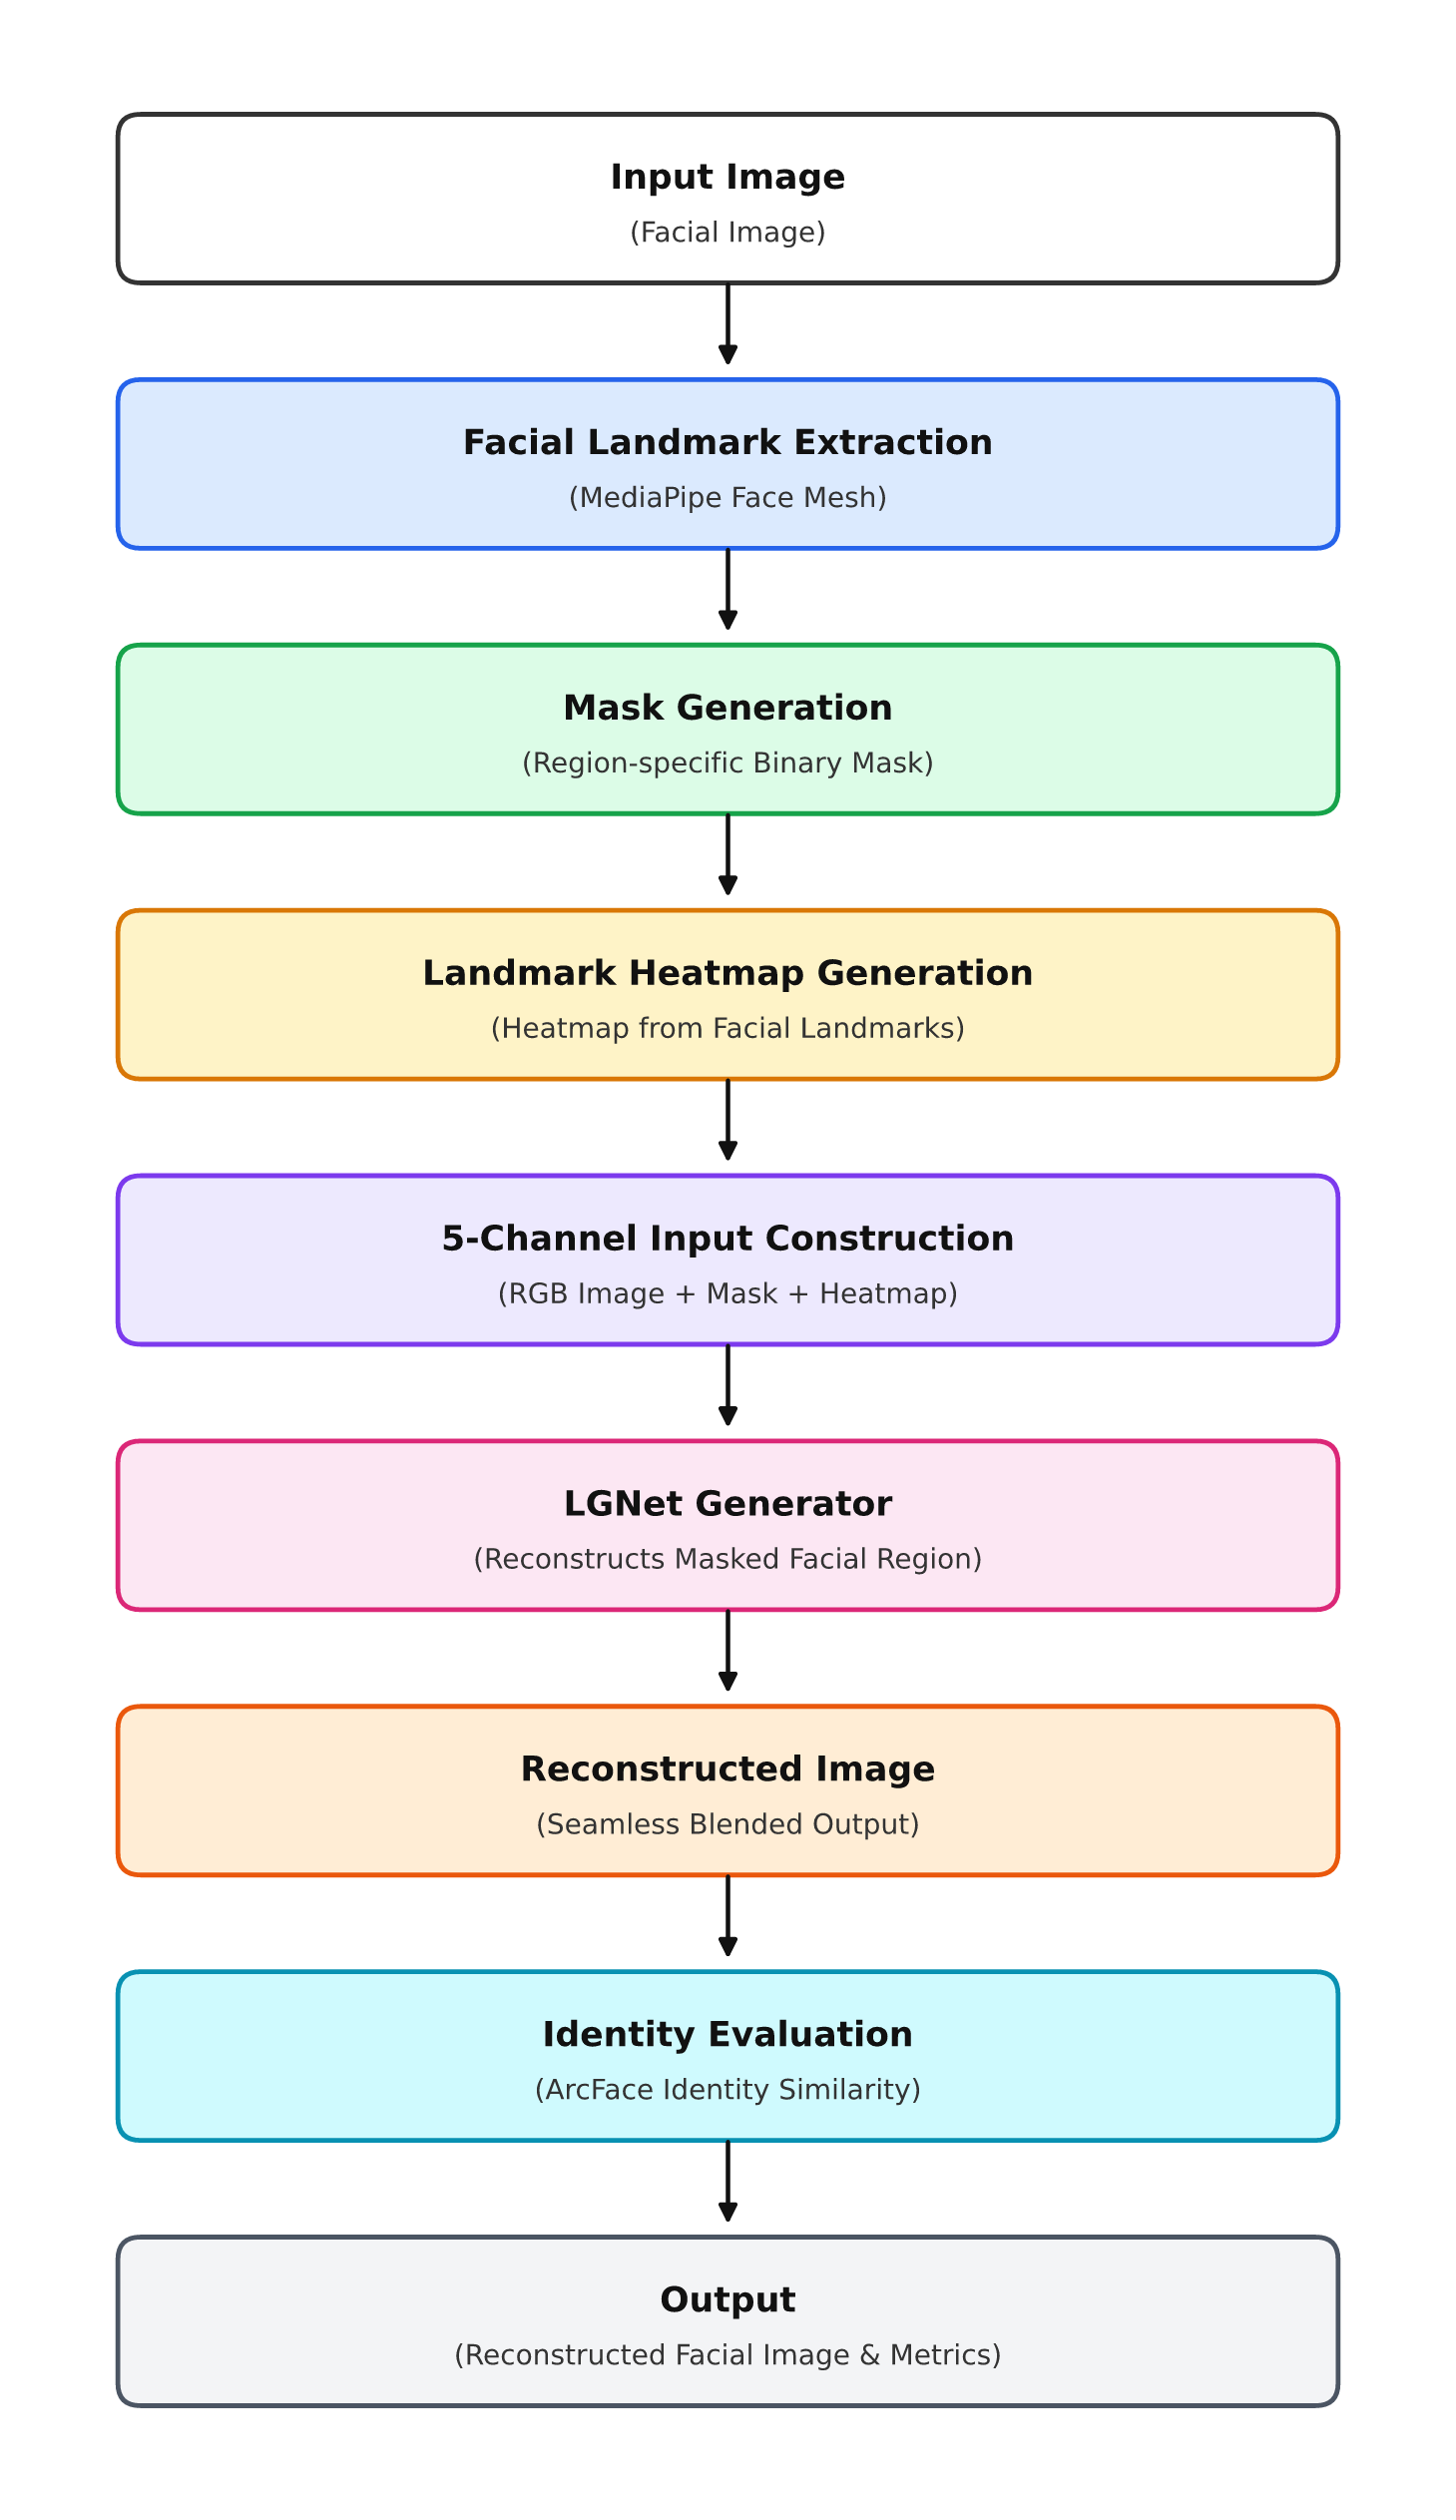
\includegraphics[width=0.85\textwidth]{img/fig3_2_clean.png}
    \caption{MorphAI model architecture}
    \label{fig:morphai_architecture}
\end{figure}

\noindent MorphAI adopts a facial inpainting architecture designed to reconstruct
selected facial regions while preserving the overall appearance and
identity of the input face. The system combines facial landmark
extraction, mask generation, landmark-based guidance, and the LGNet
generator to produce the reconstructed image.

% \begin{figure}[H]
%     \centering
%     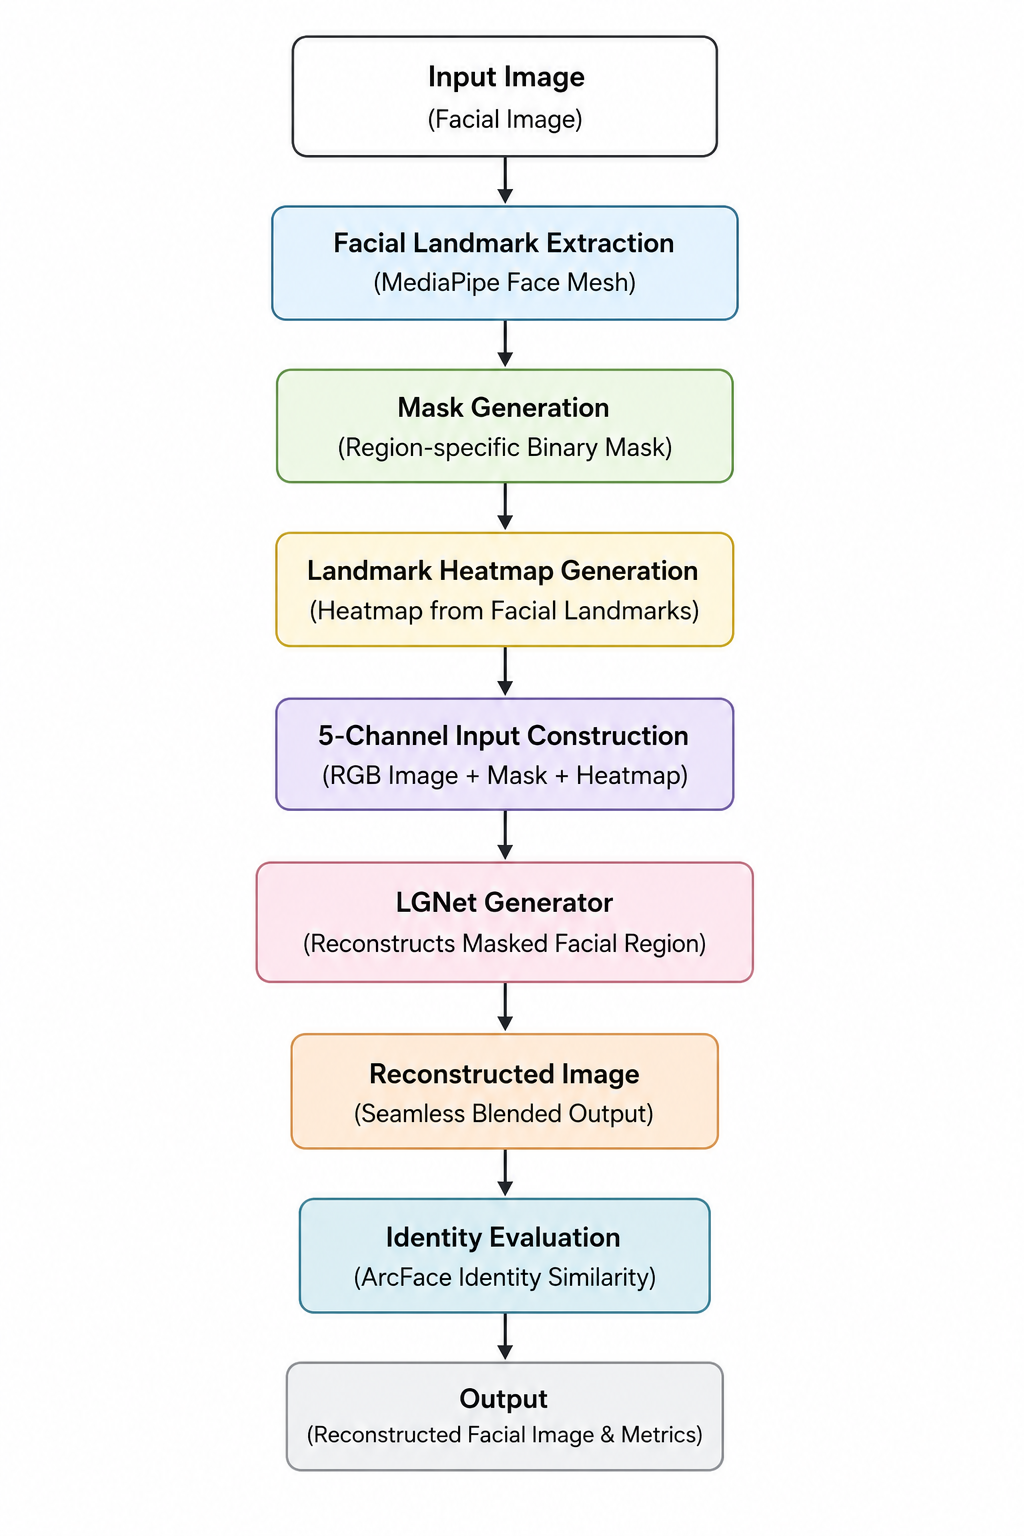
\includegraphics[width=0.85\textwidth]{img/morphai_architecture.png}
%     \caption{MorphAI model architecture}
%     \label{fig:morphai_architecture}
% \end{figure}

\subsection{Input Image}

The system receives a facial image from the user through the frontend.
The image is prepared and passed to the backend for facial region
selection and reconstruction.

\subsection{Facial Landmark Extraction}

The LandmarkExtractor detects important facial landmarks from the input
image. These landmarks provide structural information about the face
and help guide the reconstruction of the selected region.

\subsection{Mask Generation}

The MaskGenerator creates a region-specific binary mask based on the
selected facial area. The mask identifies the region to be reconstructed
while preserving the remaining facial content.

\subsection{Landmark Heatmap}

The detected landmarks are converted into a spatial heatmap. This
heatmap provides the generator with additional information about the
facial structure and location of important facial features.

\clearpage
\subsection{LGNet Generator}

The LGNetGenerator is the main reconstruction component of MorphAI. It
receives the RGB image, facial mask, and landmark-based information as
the required multi-channel input. The generator processes these inputs
and reconstructs the selected facial region while maintaining
consistency with the surrounding facial features.

\subsection{Identity Evaluation}

The reconstructed image can be evaluated using the IdentityExtractor
to determine whether the generated face maintains the identity
characteristics of the original input. This provides an additional
measure for assessing the quality of the reconstruction.

% \begin{figure}[htbp]
%     \centering
%     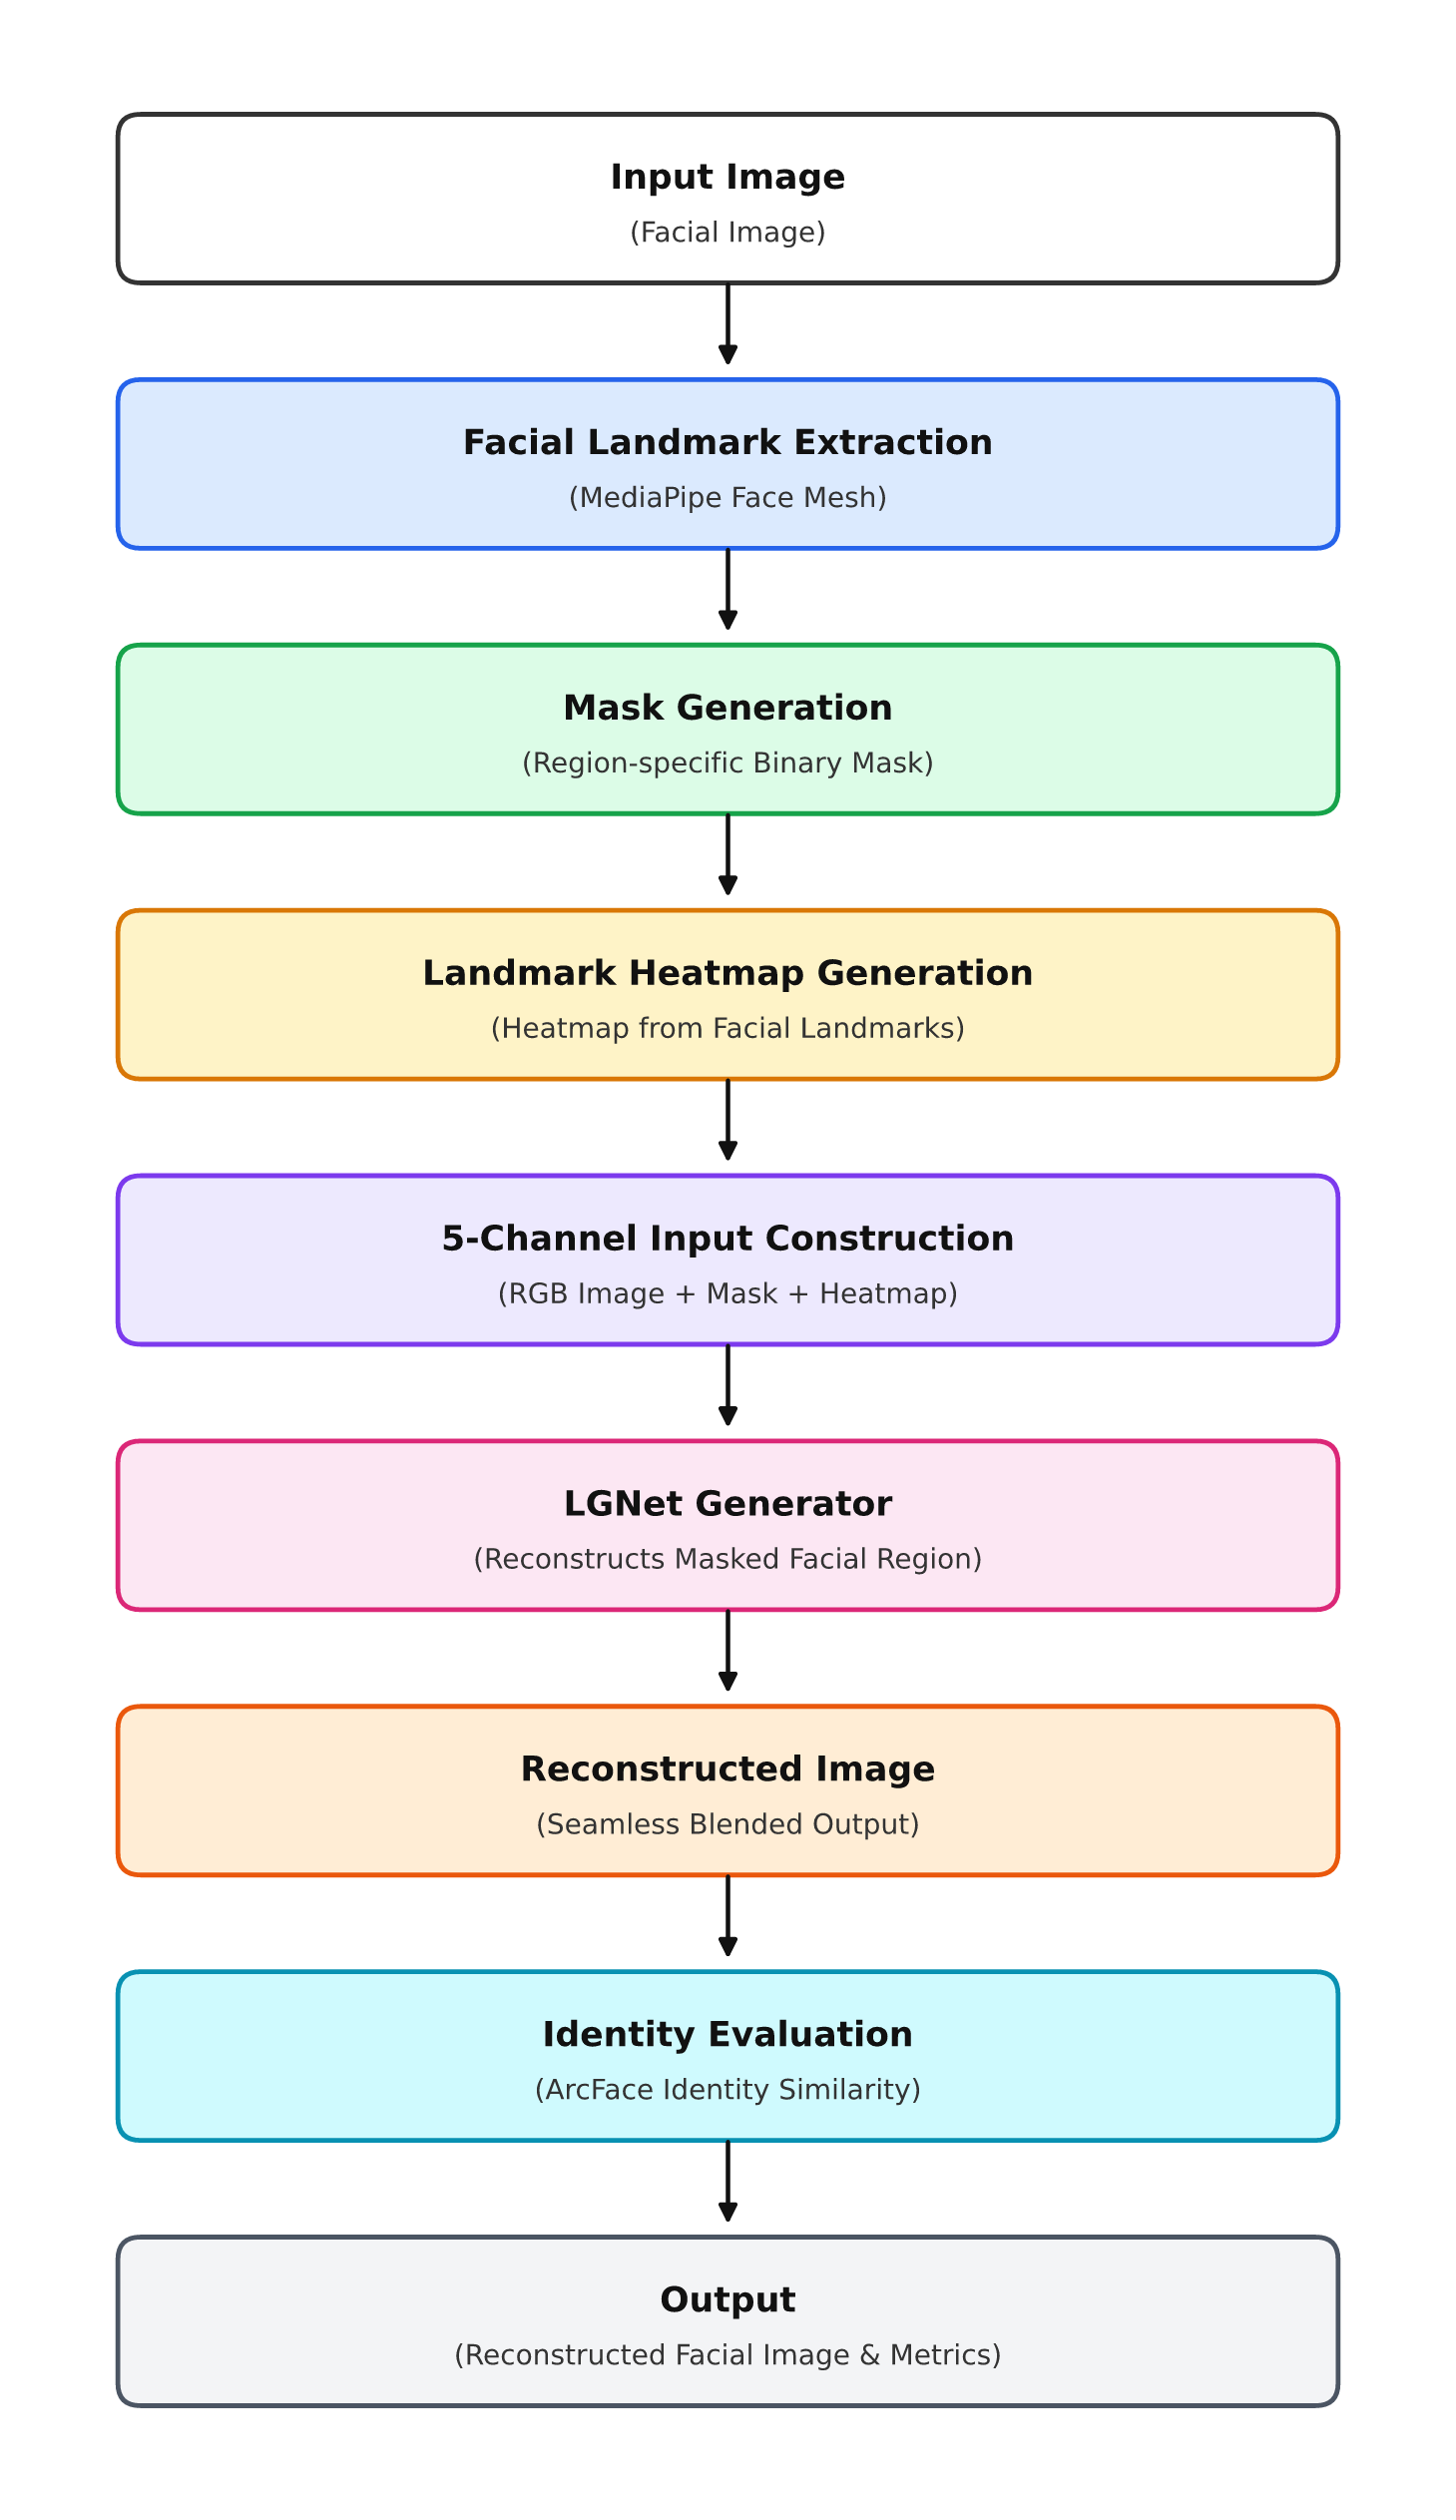
\includegraphics[width=0.85\textwidth]{img/fig3_2_clean.png}
%     \caption{MorphAI model architecture}
%     \label{fig:morphai_architecture}
% \end{figure}


% \clearpage
\subsection{Model Architecture Summary}

Table~\ref{tab:morphai_arch} summarises the main components of the
MorphAI architecture.

\begin{table}[H]
\centering
\caption{MorphAI model architecture summary}
\label{tab:morphai_arch}
\begin{tabular}{ll}
\hline
\textbf{Component} & \textbf{Purpose} \\
\hline
Frontend & Image upload and region selection \\
LandmarkExtractor & Detect facial landmarks \\
MaskGenerator & Generate the reconstruction mask \\
Landmark Heatmap & Provide facial structural guidance \\
LGNetGenerator & Reconstruct the selected facial region \\
IdentityExtractor & Evaluate identity preservation \\
\hline
\end{tabular}
\end{table}
% ────────────────────────────────────────────────────────────────────

\subsection{Technical Contribution of MorphAI}
The primary technical contribution of MorphAI is the incorporation of explicit facial 
landmark heatmap conditioning into a modified LGNet-based facial inpainting framework. Rather than introducing an entirely new generative architecture, MorphAI builds on the existing Local-Global Network (LGNet) generator and extends it with structural guidance 
derived from facial landmarks.

\noindent The model receives a five-channel input consisting of the RGB facial image (3 channels), 
a binary facial mask (1 channel), and a landmark heatmap (1 channel):
\begin{equation}
    X = [I_{RGB}, M, H] \in \mathbb{R}^{5 \times 256 \times 256}
\end{equation}

\noindent The landmark heatmap $H$ provides the generator with explicit spatial information about the position and shape of important facial features, which is not available to the 
original LGNet or to context-only inpainting models such as LaMa. This allows the 
generator to combine two complementary sources of information during reconstruction: 
the visual context surrounding the masked region, and the underlying facial geometry 
indicated by the landmarks.

\noindent In addition to landmark conditioning, MorphAI incorporates identity-preserving supervision using ArcFace-based facial embeddings during training, encouraging the reconstructed 
region to remain consistent with the identity of the input subject. This distinguishes MorphAI from landmark-based methods such asDeepFaceReshaping~\cite{chen2024deepface}, 
which use landmarks primarily to drive interactive geometric reshaping of \textit{visible} 
facial regions, rather than as a conditioning signal for reconstructing \textit{missing} 
regions.

\noindent Overall, the novelty of MorphAI lies in the combination of the following elements, 
rather than in proposing a new generative architecture:
\begin{enumerate}
    \item Landmark heatmap conditioning,
    \item Identity-preserving loss supervision, and
    \item Application of this combined approach to region-specific facial inpainting.
\end{enumerate}
MorphAI is therefore best described as a landmark-conditioned, identity-preserving 
adaptation of LGNet for facial region reconstruction.


\section{Hyperparameters}

The MorphAI model was trained using PyTorch with Automatic Mixed Precision
(autocast). The training configuration was selected to balance reconstruction
quality, facial structure, texture consistency, and identity preservation.

\begin{itemize}
    \item \textbf{Training Configuration:} The MorphAI model was trained for 5 epochs using the CelebA-HQ dataset containing 16,800 facial images. A portion of these images was held out for evaluation.
    
    \item \textbf{Loss Function:} A composite loss combining L1, perceptual,
    style, identity, and facial landmark losses was used to improve
    reconstruction quality and preserve facial characteristics.
    
    \item \textbf{L1 Loss:} Measures pixel-level differences between the
    reconstructed and target images.
    
    \item \textbf{Perceptual Loss:} Uses VGG-16 features to preserve important
    facial structures and visual details.
    
    \item \textbf{Style Loss:} Uses Gram matrix features to maintain texture
    and appearance consistency.
    
    \item \textbf{Identity Loss:} Uses facial embedding cosine similarity to
    preserve the identity of the input subject.
    
    \item \textbf{Landmark Loss:} Uses Wing loss to maintain the position and
    structure of important facial landmarks.

    \item \textbf{Adversarial Loss:} Uses a PatchGAN discriminator trained
jointly with the generator to improve the local realism and texture
fidelity of reconstructed facial regions.
    
    \item \textbf{Training Efficiency:} Automatic Mixed Precision was used
    to reduce GPU memory consumption and improve training efficiency.
    
    \item \textbf{Training Convergence:} Training loss decreased from
    0.3479 in the first epoch to 0.2774 in the fifth epoch, while validation
    loss decreased from 0.3640 to 0.2950, indicating stable convergence.
    
    \item \textbf{Final Checkpoint:} The fifth-epoch checkpoint,
    \texttt{morphai\_epoch\_05.pt}, was selected as the final model for
    evaluation and comparison with the LaMa baseline.
\end{itemize}

% \noindent Table~\ref{tab:hparams} summarizes the main training configuration.

\begin{table}[H]
\centering
\caption{Training configuration of the proposed LGNet model}
\label{tab:hparams}
\renewcommand{\arraystretch}{1.3}
\begin{tabular}{|l|l|}
\hline
\textbf{Training Setting} & \textbf{Value} \\ \hline
Framework & PyTorch \\ \hline
Training method & Automatic Mixed Precision (autocast) \\ \hline
Training epochs & 5 \\ \hline
% Dataset size & 28,000 facial images \\ \hline
Dataset & CelebA-HQ (16,800 facial images) \\ \hline
Loss function & Composite multi-objective loss \\ \hline
Pixel loss & L1 loss \\ \hline
Perceptual loss & VGG-16 based \\ \hline
Style loss & Gram matrix based \\ \hline
Adversarial loss    PatchGAN discriminator\\ \hline
Identity loss & Face embedding cosine loss \\ \hline
Landmark loss & Wing loss \\ \hline
Final checkpoint & \texttt{morphai\_epoch\_05.pt} \\ \hline
\end{tabular}
\end{table}

\section{Performance Evaluation Metrics}

MorphAI is evaluated using metrics that measure reconstruction quality,
visual similarity, and identity preservation. The evaluation was performed
using 2,800 held-out facial images. For each held-out image, six
facial-region masks were generated for the left eyebrow, right eyebrow,
left eye, right eye, nose, and mouth. Therefore, the evaluation consisted
of $2,800 \times 6 = 16,800$ region-specific evaluation samples. These
16,800 samples are derived evaluation instances and do not represent
16,800 unique facial images.

\subsection{Peak Signal-to-Noise Ratio (PSNR)}

PSNR measures the pixel-level similarity between the reconstructed image and the original image. A higher PSNR value indicates that the reconstructed image is closer to the ground-truth image.

\begin{equation}
\text{PSNR} =
10\log_{10}\left(\frac{MAX_I^2}{\text{MSE}}\right)
\end{equation}

\noindent where $MAX_I$ is the maximum possible pixel value and MSE is the mean squared error.

\subsection{Structural Similarity Index (SSIM)}

SSIM measures how similar the structure of the reconstructed image is to the original image. It considers factors such as brightness, contrast, and structural information. Higher SSIM indicates better structural similarity.

\subsection{Learned Perceptual Image Patch Similarity (LPIPS)}

LPIPS measures perceptual similarity using features extracted from a deep neural network. It is useful for checking whether the reconstructed facial region looks visually similar to the original. Lower LPIPS values indicate better perceptual similarity.

\subsection{Fréchet Inception Distance (FID)}

FID compares the feature distributions of generated and real images. It is mainly used to measure the realism of generated images. A lower FID value indicates that the generated images are closer to real facial images.

\subsection{Identity Similarity}

Identity similarity measures whether the reconstructed face still represents the same person as the original image. MorphAI uses facial embeddings and cosine similarity for this evaluation.

\begin{equation}
\text{Identity Similarity} =
\frac{f(\hat{I}) \cdot f(I)}
{\|f(\hat{I})\|_2 \|f(I)\|_2}
\end{equation}

\noindent where $f(I)$ and $f(\hat{I})$ represent the facial embeddings of the original and reconstructed images, respectively. Higher similarity indicates better identity preservation.

\subsection{Root Mean Square Error (RMSE)}

RMSE measures the average pixel-level difference between the reconstructed image and the ground-truth image. Lower RMSE indicates smaller reconstruction errors.

\begin{equation}
\text{RMSE} =
\sqrt{
\frac{1}{CHW}
\sum_{c=1}^{C}
\sum_{h=1}^{H}
\sum_{w=1}^{W}
\left(\hat{I}_{c,h,w}-I_{c,h,w}\right)^2
}
\end{equation}

\noindent where $\hat{I}$ is the reconstructed image and $I$ is the ground-truth image.

\subsection{RMSE-log}

RMSE-log measures the reconstruction error after applying a logarithmic
transformation to the pixel values. It reduces the influence of large
pixel differences and provides an error measure on a logarithmic scale.

\noindent The RMSE-log is defined as:

\label{sec:rmse-log}
\begin{equation}
RMSE_{\log} =
\sqrt{
\frac{1}{CHW}
\sum_{c=1}^{C}
\sum_{h=1}^{H}
\sum_{w=1}^{W}
\left[
\log(1+\hat{I}_{c,h,w})
-
\log(1+I_{c,h,w})
\right]^2
}
\label{eq:rmse-log}
\end{equation}

\noindent where $I$ represents the ground-truth image, $\hat{I}$ represents the
reconstructed image, $C$ is the number of image channels, and $H$ and
$W$ are the image height and width, respectively. The $\log(1+x)$
transformation allows zero-valued pixels to be handled safely.

\noindent Lower RMSE-log values indicate smaller reconstruction errors and
therefore better reconstruction quality.
 
\section{Model Variants Explored}

Different inpainting configurations were evaluated during the development
of MorphAI. LaMa was used as a pretrained baseline, while LGNet was used
as the main inpainting model. A modified LGNet configuration was then
developed by providing RGB images together with a binary facial mask and
landmark heatmap. The main variants are summarized in
Table~\ref{tab:model_variants_ch3}, while their quantitative results are
presented in Section~5.1.

\begin{table}[h!]
\centering
\renewcommand{\arraystretch}{1.4}
\begin{tabular}{|l|p{9cm}|}
\hline
\textbf{Variant} & \textbf{Description} \\ \hline

LaMa & Pretrained image inpainting model. \\ \hline

LGNet & Inpainting model used for facial reconstruction. \\ \hline

\textbf{LGNet + 5-channel input} &
\textbf{Modified LGNet using RGB image, binary facial mask, and landmark
heatmap for guided facial reconstruction.} \\ \hline

\end{tabular}
\caption{Model variants explored during MorphAI development}
\label{tab:model_variants_ch3}
\end{table}
    \chapter{SYSTEM DESIGN}

\section{Requirement Specification}

\subsection{Functional Requirements}

The proposed MorphAI system shall provide the following functional requirements:

\begin{itemize}
\item \textbf{Input Handling:} The system shall accept facial images from the CelebA-HQ dataset for training and evaluation.

\item \textbf{Image Pre-processing:} The system shall resize input facial images to $256 \times 256$ pixels and prepare them for the reconstruction pipeline.

\item \textbf{Facial Landmark Detection:} The system shall use MediaPipe Face Mesh to detect facial landmarks from the input image.

\item \textbf{Mask Generation:} The system shall generate facial masks for selected regions using semantic facial regions and random rectangular masks.

\item \textbf{Landmark Heatmap Generation:} The system shall convert the detected facial landmarks into a landmark heatmap to provide additional facial structure information.

\item \textbf{Model Input Preparation:} The system shall combine the three RGB channels, one binary mask channel, and one landmark heatmap channel to create a five-channel input of size $5 \times 256 \times 256$.

\item \textbf{Facial Reconstruction:} The system shall use the modified LGNet generator to reconstruct the masked facial regions and produce a $256 \times 256$ RGB facial image.

\item \textbf{Identity Preservation:} The system shall use a pretrained facial recognition model to calculate identity loss and encourage the reconstructed image to preserve the identity of the input subject.

\item \textbf{Model Training:} The system shall train the modified LGNet using a composite loss consisting of reconstruction, perceptual, style, identity, and adversarial objectives.

\item \textbf{Evaluation:} The system shall evaluate reconstructed images using image-quality and identity-based metrics, including PSNR, SSIM, LPIPS, FID, RMSE, RMSE-log, and identity similarity.

\item \textbf{Inference:} The system shall accept a facial image and generate a reconstructed facial image using the trained MorphAI model.

\item \textbf{Output:} The system shall provide the reconstructed facial image while preserving the visible facial structure and attempting to maintain the identity of the subject.
\end{itemize}

\subsection{Non-Functional Requirements}

The MorphAI system should satisfy the following non-functional requirements:

\begin{itemize}
\item \textbf{Performance:} The system should use GPU acceleration to reduce model training and inference time.

\item \textbf{Accuracy:} The system should generate realistic facial reconstructions while maintaining high structural and identity similarity.

\item \textbf{Reliability:} The preprocessing and reconstruction pipeline should produce consistent results for valid facial images and different masking conditions.

\item \textbf{Robustness:} The system should handle variations in facial expression, pose, lighting, and masked facial regions as effectively as possible.

\item \textbf{Usability:} The system should provide a simple pipeline for preparing facial images, generating reconstructions, and evaluating the results.

\item \textbf{Maintainability:} The system should use modular components for preprocessing, landmark detection, mask generation, model training, inference, and evaluation so that individual components can be modified or improved easily.

\item \textbf{Scalability:} The framework should allow future experiments with larger datasets, different facial reconstruction models, and additional identity-preservation methods.

\item \textbf{Resource Efficiency:} The system should be capable of training and testing within the available GPU and memory resources without requiring specialized 3D facial scanning hardware.
\end{itemize}
\newpage

\section{Use Case Diagram}
      The Use Case Diagram \ref{fig:use case diagram} illustrates the interaction between the user and the MorphAI Facial Appearance Transformation System.
    \begin{figure}[H]
        \centering
        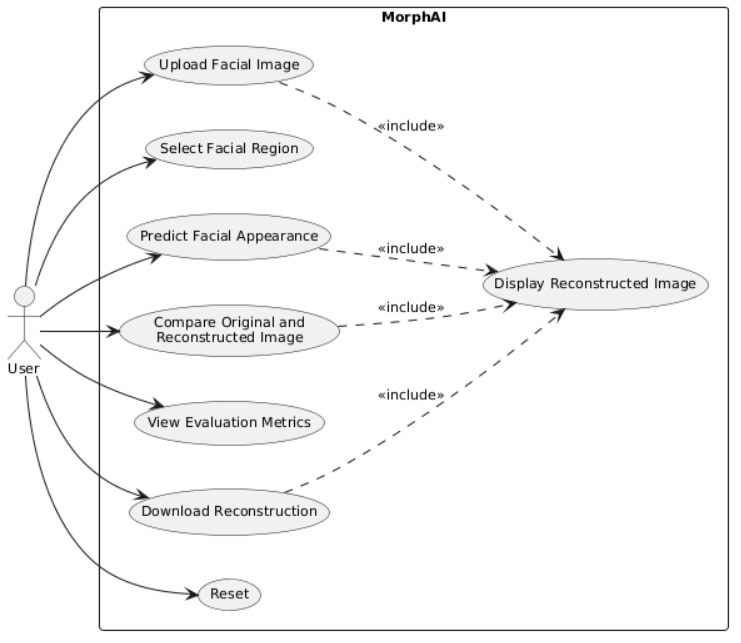
\includegraphics[scale=0.5]{img/usecase.png}
        \caption{Use Case Diagram of MorphAI}
        \label{fig:use case diagram}
   \end{figure}
     \noindent The process begins when the user uploads a facial image and selects the facial region to be reconstructed. The user can then generate a facial appearance prediction, after which the reconstructed image is displayed. The user can compare the original and reconstructed images, view evaluation metrics, download the reconstruction, or reset the prediction.
%\section{Activity Diagram}
   % \begin{figure}[H]
      %  \centering
        %\includegraphics[scale=0.69]{img/ActivityDiagram.png}
       % \caption{Activity Diagram}
       % \label{fig:activity diagram}
  % \end{figure}
 %  The activity diagram illustrates the complete workflow of the system from start to finish. The process begins when the user uploads a handwritten image. If the image format is invalid, an error message is displayed and the process terminates. If the format is valid, the image preview is shown and the image enters the preprocessing pipeline, which consists of grayscale conversion, binarization, deskewing, and tight cropping. The preprocessed image is then fed into the fine-tuned TrOCR model to generate Unicode Nepali text. The post-processing stage runs in parallel to display the recognized word, generate a character-level confidence breakdown, and produce a pipeline processing log. Finally, if the user chooses to export the result, they can either download it as a .txt file or copy it to the clipboard, after which the process ends.

\newpage
\section{Class Diagram for System}
This class diagram \ref{fig:classdiagram} illustrates the structure and
relationships among the major components of the MorphAI facial inpainting
system.

\begin{figure}[H]
    \centering
    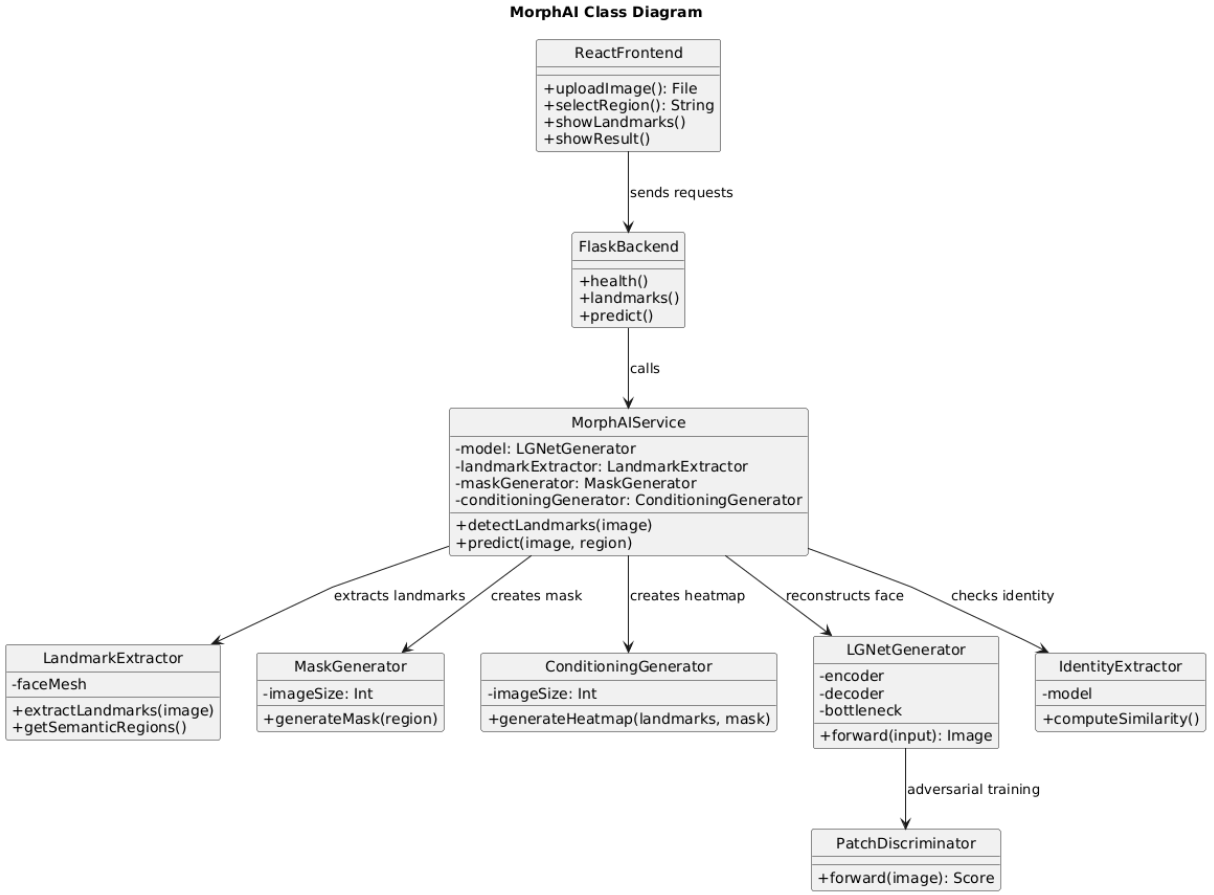
\includegraphics[scale=0.5]{img/class_diagram.png}
    \caption{Class diagram of MorphAI system}
    \label{fig:classdiagram}
\end{figure}
 \noindent The \textbf{ReactFrontend} serves as the entry point where the user uploads a facial image, selects the target facial region, and views the reconstructed result. It communicates with the \textbf{FlaskBackend}, which handles health checks, landmark extraction, and prediction requests. The \textbf{MorphAIService} coordinates the main processing components, including the \textbf{LandmarkExtractor}, \textbf{MaskGenerator}, \textbf{ConditioningGenerator}, \textbf{LGNetGenerator}, and \textbf{IdentityExtractor}. The \textbf{LandmarkExtractor} detects facial landmarks and semantic regions, while the \textbf{MaskGenerator} creates the mask for the selected facial region. The \textbf{ConditioningGenerator} uses the extracted landmarks and mask to generate the conditioning heatmap. These inputs are provided to the \textbf{LGNetGenerator}, which reconstructs the masked facial region using its encoder, decoder, and bottleneck components. The generated image is further evaluated through the \textbf{PatchDiscriminator} during adversarial training and the \textbf{IdentityExtractor} to verify identity preservation. Each component has a well-defined responsibility, providing a structured flow from facial image input and region selection to reconstructed and identity-preserving facial output.



  
%\section{Class Diagram for Data }

%\section{Database Schema}

\section{Sequence Diagram}
    \begin{figure}[H]
        \centering
        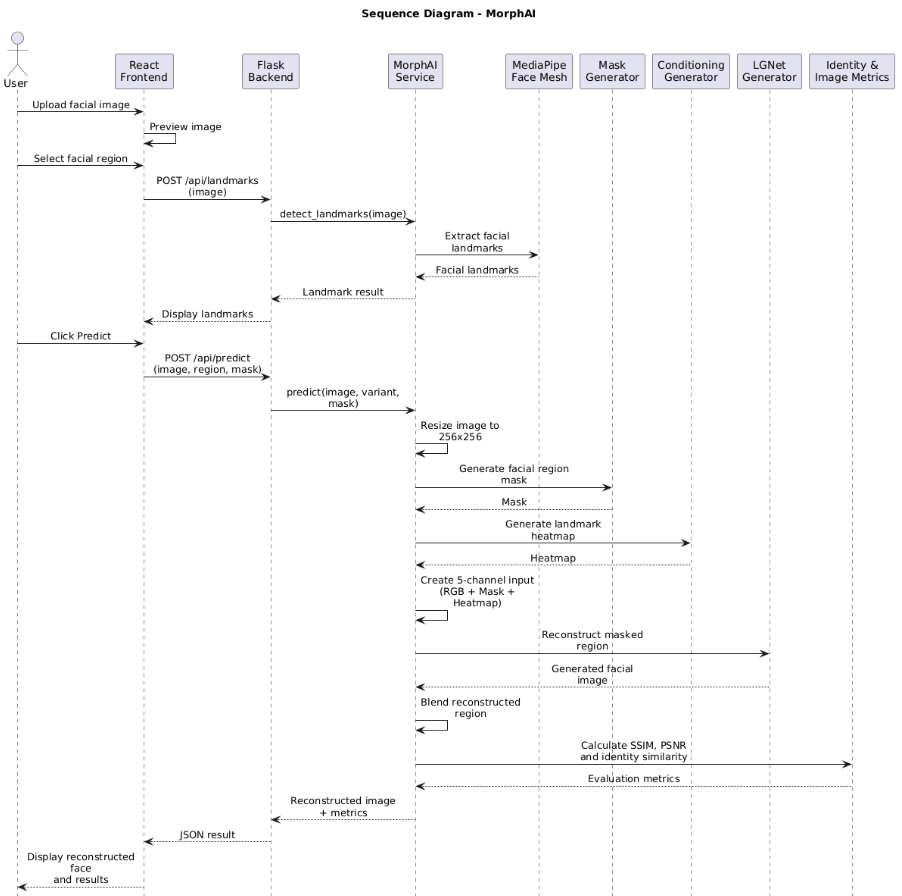
\includegraphics[scale=0.65]{img/activity_diagram.png}
        \caption{Sequence Diagram of MorphAI system}
        \label{fig:sequence diagram}
   \end{figure}

\clearpage
\noindent The sequence diagram \ref{fig:sequence diagram} illustrates the interaction between system components during facial inpainting. The user uploads an image and selects a facial region through the React frontend. The Flask backend forwards the request to the MorphAIService, which extracts landmarks, generates a mask and heatmap, and forms the five-channel input for the LGNetGenerator. The generated facial image is then returned to the frontend for display, while the IdentityExtractor evaluates identity preservation.
\newline
\noindent The backend then sends the image to the MorphAIService, which generates the facial mask, landmark heatmap, and five-channel input for the LGNetGenerator. The reconstructed image is blended and evaluated using SSIM, PSNR, and identity similarity before being returned to the frontend and displayed to the user.
   %  \begin{figure}[H]
   %      \centering
   %      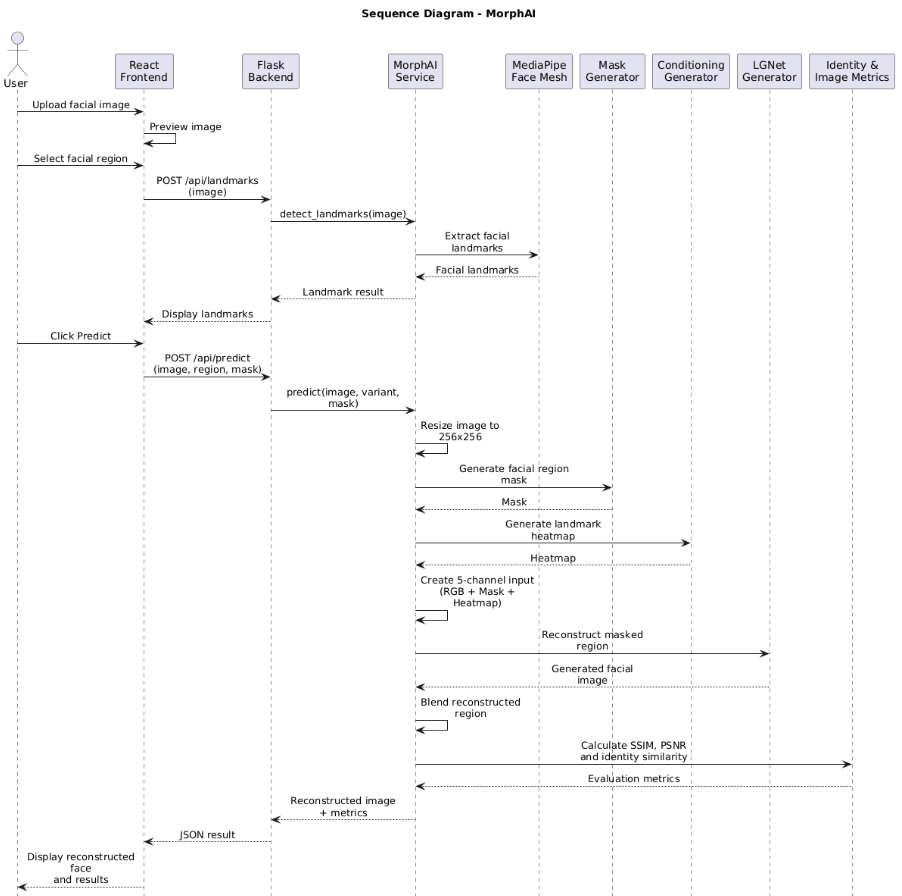
\includegraphics[scale=0.65]{img/activity_diagram.png}
   %      \caption{Sequence Diagram of MorphAI system}
   %      \label{fig:sequence diagram}
   % \end{figure}


%\section{Data Flow Diagram}

   % \begin{figure}[H]
      %  \centering
       % \includegraphics[scale=0.38]{img/dfd0.png}
       % \caption{Level 0 Data Flow Diagram}
       % \label{fig:Level 0 Data Flow Diagram}
  % \end{figure}
  % The context diagram provides a high-level overview of the system. The user provides a handwritten image as input to the Nepali Handwritten Word Recognition System. The system processes the image and returns the recognized Unicode Nepali text, downloadable output, and confidence logs back to the user. Any invalid image format triggers an error notification.

   % \begin{figure}[H]
      %  \centering
       % \includegraphics[scale=0.5]{img/Level1.jpg}
      %  \caption{Level 1 Data Flow Diagram}
       % \label{fig:Level 1 Data Flow Diagram}
   %\end{figure}
%\noindent
%The Level 1 Data Flow Diagram breaks down the internal processes of the system. The user submits a handwritten image which enters the Upload Image process. The raw image is then passed to the Preprocess Image process where it is cleaned and normalized. The cleaned image is fed into the Run TrOCR Inference process, which loads model weights from the TrOCR Model data store. The generated token IDs are passed to the Decode Output process, which references the Nepali Tokenizer data store to map tokens to Unicode characters. The resulting Unicode text is then passed to the Display Result process, which returns the recognized word and character breakdown to the user.





%\section{Deployment Diagram}
%\textbf{Note: All the diagram is not mandatory..select according to the type of project you are going to do.}
    \chapter{RESULT AND DISCUSSION}


\section{Experiment Setup}

All experiments for the proposed MorphAI system were conducted using a
PyTorch-based deep learning environment with GPU acceleration. The model
was trained using Automatic Mixed Precision (AMP) to improve computational
efficiency and reduce GPU memory usage. Training was performed for five
epochs on a dataset containing more than 16,800 facial images. Table
~\ref{tab:hardware} summarises the hardware and software environment used
for model training and evaluation.

\begin{table}[h!]
\centering
\renewcommand{\arraystretch}{1.1}
\begin{tabular}{|l|l|}
\hline
\textbf{Component} & \textbf{Specification} \\ \hline
GPU & NVIDIA GeForce RTX 4050 Laptop GPU (6 GB VRAM) \\ \hline
System RAM & 16 GB \\ \hline
Operating System & Windows 11 Home \\ \hline
Python & 3.11.9 \\ \hline
PyTorch & 2.6.0 + CUDA 12.4 \\ \hline
Training Precision & Automatic Mixed Precision (AMP) \\ \hline
Training Epochs & 5 \\ \hline
Training Dataset & 16,800 facial images \\ \hline
\end{tabular}
\vspace{2pt}
\caption{Hardware and software environment used for MorphAI}
\label{tab:hardware}
\end{table}

\section{Training Configuration}
The proposed MorphAI model was trained using the modified LGNet generator
with landmark-based structural conditioning. The input image was resized
to $256 \times 256$ pixels and combined with a facial mask and landmark
heatmap to form a five-channel input. The model was trained using GPU
acceleration and Automatic Mixed Precision (AMP). The main training
configuration is summarised in Table~\ref{tab:training_config}.
% \clearpage
\begin{table}[H]
\centering
\renewcommand{\arraystretch}{1.3}
\begin{tabular}{|l|l|}
\hline
\textbf{Training Setting} & \textbf{Value} \\ \hline
Dataset & CelebA-HQ (16,800 original images) \\ \hline
Image Resolution & $256 \times 256$ \\ \hline
Model & Modified LGNet Generator \\ \hline
Input & 5-channel (RGB + Mask + Heatmap) \\ \hline
Training Epochs & 5 \\ \hline
Training Precision & Automatic Mixed Precision (AMP) \\ \hline
Training Mask & Semantic facial-region masks \\ \hline
Inference Mask & Semantic masks \\ \hline
Evaluation & PSNR, SSIM, LPIPS, FID, RMSE-log, Identity Similarity \\ \hline
\end{tabular}
\caption{Training configuration of the proposed MorphAI model}
\label{tab:training_config}
\end{table}

\noindent The model was trained for five epochs primarily due to the
computational constraints of the available hardware. Training was
performed on a single NVIDIA RTX 4050 Laptop GPU (6\,GB VRAM), using
Automatic Mixed Precision (AMP) to reduce GPU memory usage and improve
computational efficiency within this resource budget. The training and
validation losses decreased consistently throughout training, indicating
stable convergence. The loss values obtained during training are
presented in Table~\ref{tab:training_loss}.

\begin{table}[H]
\centering
\renewcommand{\arraystretch}{1.2}
\begin{tabular}{|c|c|c|c|}
\hline
\textbf{Epoch} & \textbf{Training Loss} & \textbf{Validation Loss} &
\textbf{Loss Gap} \\ \hline
1 & 0.3479 & 0.3640 & 0.0161 \\ \hline
2 & 0.3124 & 0.3284 & 0.0160 \\ \hline
3 & 0.3003 & 0.3167 & 0.0164 \\ \hline
4 & 0.2847 & 0.2983 & 0.0136 \\ \hline
5 & 0.2774 & 0.2950 & 0.0176 \\ \hline
\end{tabular}
\caption{Training and validation loss across five epochs}
\label{tab:training_loss}
\end{table}

\noindent The training loss decreased from 0.3479 to 0.2774, while the
validation loss decreased from 0.3640 to 0.2950. The relatively small and
stable training--validation gap (ranging from 0.0136 to 0.0176) indicates
stable training without a substantial increase in validation error,
suggesting the model had not begun overfitting by the fifth epoch. Based
on this consistent convergence behaviour and the available computational
budget, the fifth-epoch checkpoint was selected as the final model for
evaluation. Training was not extended beyond five epochs, so no claim is
made regarding whether additional epochs would have produced further
improvement or diminishing returns.

\subsection{Ablation Consideration: Landmark Heatmap Conditioning}
The contribution of landmark heatmap conditioning is discussed based on the model 
architecture and the overall reconstruction results reported in this chapter, rather 
than through a separate controlled experiment. A dedicated ablation study — training 
an identical LGNet variant without the landmark heatmap channel, under the same 
dataset, epoch budget, and evaluation protocol — was not conducted for this project 
due to GPU and time constraints (a single 6\,GB VRAM GPU and a five-epoch training 
budget). The comparison against the LaMa baseline in Table 5.5, which does not use 
landmark conditioning at all, offers indirect evidence that the added structural 
guidance contributes to MorphAI's stronger PSNR, SSIM, and identity-similarity scores, 
but a same-architecture, single-variable ablation is left as future work.

\subsection{Quantitative Evaluation}

Semantic region-wise evaluation was performed on six facial regions
using the same 2,800 held-out facial images. Each image was evaluated
with respect to each of the six facial regions, resulting in
$2,800 \times 6 = 16,800$ region-specific evaluation samples. As shown in Table~\ref{tab:semantic_region},
LGNet generally achieves higher PSNR, SSIM, identity similarity, and lower
RMSE-log and FID than LaMa. LGNet also shows particularly strong performance
for the mouth and eye regions. LPIPS is lower for LaMa in several regions,
indicating that LGNet does not outperform the baseline on every metric.
Overall, the results demonstrate strong structural and identity preservation
by the proposed LGNet model.

\begin{table}[H]
\centering
\renewcommand{\arraystretch}{1.25}
\resizebox{\textwidth}{!}{%
\begin{tabular}{|l|l|c|c|c|c|c|c|}
\hline
\textbf{Region} & \textbf{Model} & \textbf{PSNR $\uparrow$} &
\textbf{SSIM $\uparrow$} & \textbf{LPIPS $\downarrow$} &
\textbf{ArcFace ID $\uparrow$} & \textbf{RMSE-log $\downarrow$} &
\textbf{FID $\downarrow$} \\ \hline

Left Eyebrow & LGNet & 42.36 dB & 0.9932 & 0.0061 & 0.9880 & 0.0058 & 0.2439 \\ \hline
Left Eyebrow & LaMa  & 42.10 dB & 0.9812 & 0.0025 & 0.9726 & 0.0061 & 0.1581 \\ \hline

Right Eyebrow & LGNet & 42.27 dB & 0.9931 & 0.0062 & 0.9869 & 0.0059 & 0.2422 \\ \hline
Right Eyebrow & LaMa  & 42.03 dB & 0.9811 & 0.0026 & 0.9690 & 0.0062 & 0.1549 \\ \hline

Left Eye & LGNet & 41.17 dB & 0.9938 & 0.0051 & 0.9966 & 0.0067 & 0.2491 \\ \hline
Left Eye & LaMa  & 39.97 dB & 0.9819 & 0.0032 & 0.9880 & 0.0083 & 0.7603 \\ \hline

Right Eye & LGNet & 41.14 dB & 0.9938 & 0.0051 & 0.9963 & 0.0067 & 0.2401 \\ \hline
Right Eye & LaMa  & 40.05 dB & 0.9819 & 0.0031 & 0.9869 & 0.0082 & 0.6960 \\ \hline

Mouth & LGNet & 39.87 dB & 0.9947 & 0.0032 & 0.9886 & 0.0081 & 0.5940 \\ \hline
Mouth & LaMa  & 34.59 dB & 0.9734 & 0.0090 & 0.9497 & 0.0142 & 2.3734 \\ \hline

Nose & LGNet & 39.09 dB & 0.9882 & 0.0092 & 0.9353 & 0.0080 & 0.7947 \\ \hline
Nose & LaMa  & 37.53 dB & 0.9754 & 0.0077 & 0.8660 & 0.0094 & 1.1818 \\ \hline

\end{tabular}%
}
\caption{Semantic region-wise evaluation of MorphAI (LGNet) and LaMa on 2,800 samples per region}
\label{tab:semantic_region}
\end{table}

\noindent The final model was evaluated using pixel-level, perceptual, and identity
metrics. The evaluation results were stored in JSON files, including
\texttt{metrics.json}. A separate set of results was generated
for comparison with the LaMa baseline.

\begin{table}[H]
\centering
\renewcommand{\arraystretch}{1.3}
\begin{tabular}{|l|c|c|}
\hline
\textbf{Metric} & \textbf{MorphAI (LGNet)} & \textbf{LaMa} \\ \hline
PSNR $\uparrow$ & 40.99 dB & 39.38 dB \\ \hline
SSIM $\uparrow$ & 0.9928 & 0.9792 \\ \hline
LPIPS $\downarrow$ & 0.0058 & 0.0047 \\ \hline
Identity Similarity $\uparrow$ & 0.9819 & 0.9554 \\ \hline
RMSE-log $\downarrow$ & 0.0069 & 0.0087 \\ \hline
FID $\downarrow$ & 0.1398 & 0.2466 \\ \hline
\end{tabular}
\caption{Quantitative comparison between MorphAI and LaMa}
\label{tab:morphai_lama}
\end{table}

\noindent MorphAI outperforms the LaMa baseline on PSNR, SSIM, identity similarity, 
RMSE-log, and FID, while LaMa achieves a slightly lower LPIPS score. Overall, these 
results indicate that the proposed landmark-conditioned LGNet provides strong 
reconstruction quality while maintaining facial identity.

\subsection{Discussion of LPIPS and Identity Preservation}
MorphAI does not outperform LaMa on every evaluation metric. LaMa achieves a slightly 
lower LPIPS score (0.0047 vs. 0.0058), indicating a lower perceptual feature distance 
according to the LPIPS metric. However, MorphAI achieves better PSNR, SSIM, ArcFace 
identity similarity, RMSE-log, and FID. This indicates that MorphAI provides stronger 
pixel-level reconstruction, structural consistency, and identity preservation, while 
LaMa has an advantage according to LPIPS.

\noindent This difference can be explained by what each metric is actually sensitive to. PSNR 
and SSIM measure pixel-level and structural similarity directly against the ground-truth 
image, and both reward MorphAI's landmark-conditioned reconstructions for closely 
matching the original facial structure. ArcFace identity similarity specifically rewards 
preservation of identity-discriminative features, which MorphAI's identity loss directly 
optimizes for during training. LPIPS, in contrast, measures similarity in a learned deep 
perceptual feature space that is more sensitive to fine-grained texture and stylistic 
detail than to precise structural or identity accuracy. It is likely that MorphAI's 
landmark and identity losses push the generator toward structurally and identity-accurate 
reconstructions, which can slightly reduce fine textural variation compared to LaMa's 
purely context-driven inpainting -- a difference LPIPS is more sensitive to than PSNR 
or SSIM.

\noindent The region-wise results in Table~\ref{tab:semantic_region} support this discussion. In the 
mouth region, for example, MorphAI achieves 39.87\,dB PSNR, 0.9947 SSIM, and 0.9886 
identity similarity, compared with LaMa's 34.59\,dB, 0.9734, and 0.9497, respectively. 
Therefore, the results demonstrate a metric-specific trade-off rather than universal 
superiority of one model: MorphAI prioritizes structural and identity fidelity, while 
LaMa's context-based inpainting produces marginally lower LPIPS distance in some regions.

\noindent Region-wise evaluation was also performed for the eyes, eyebrows, nose, and 
mouth. These results are stored in the \texttt{lama\_comparison} JSON files and provide 
additional analysis of performance across different facial regions.


\section{Software Development Approach}

\noindent The MorphAI project follows the Agile Software Development Life
Cycle (SDLC), where development is carried out through iterative stages.
Each iteration involves planning, implementation, testing, review, and
refinement. This approach allows individual components to be developed
and improved based on intermediate experimental results.

\noindent The development began with literature review, dataset
preparation, image preprocessing, and facial landmark extraction.
Subsequent iterations focused on facial mask generation, landmark
heatmap conditioning, LGNet architecture modification, and ArcFace
identity-preservation integration. The final stages focus on model
training, evaluation, comparison, and refinement. Agile was selected
because the project involves continuous experimentation with the
dataset, model architecture, and loss functions, allowing changes to be
made incrementally without affecting the entire system.
    \begin{figure}[H]
        \centering
        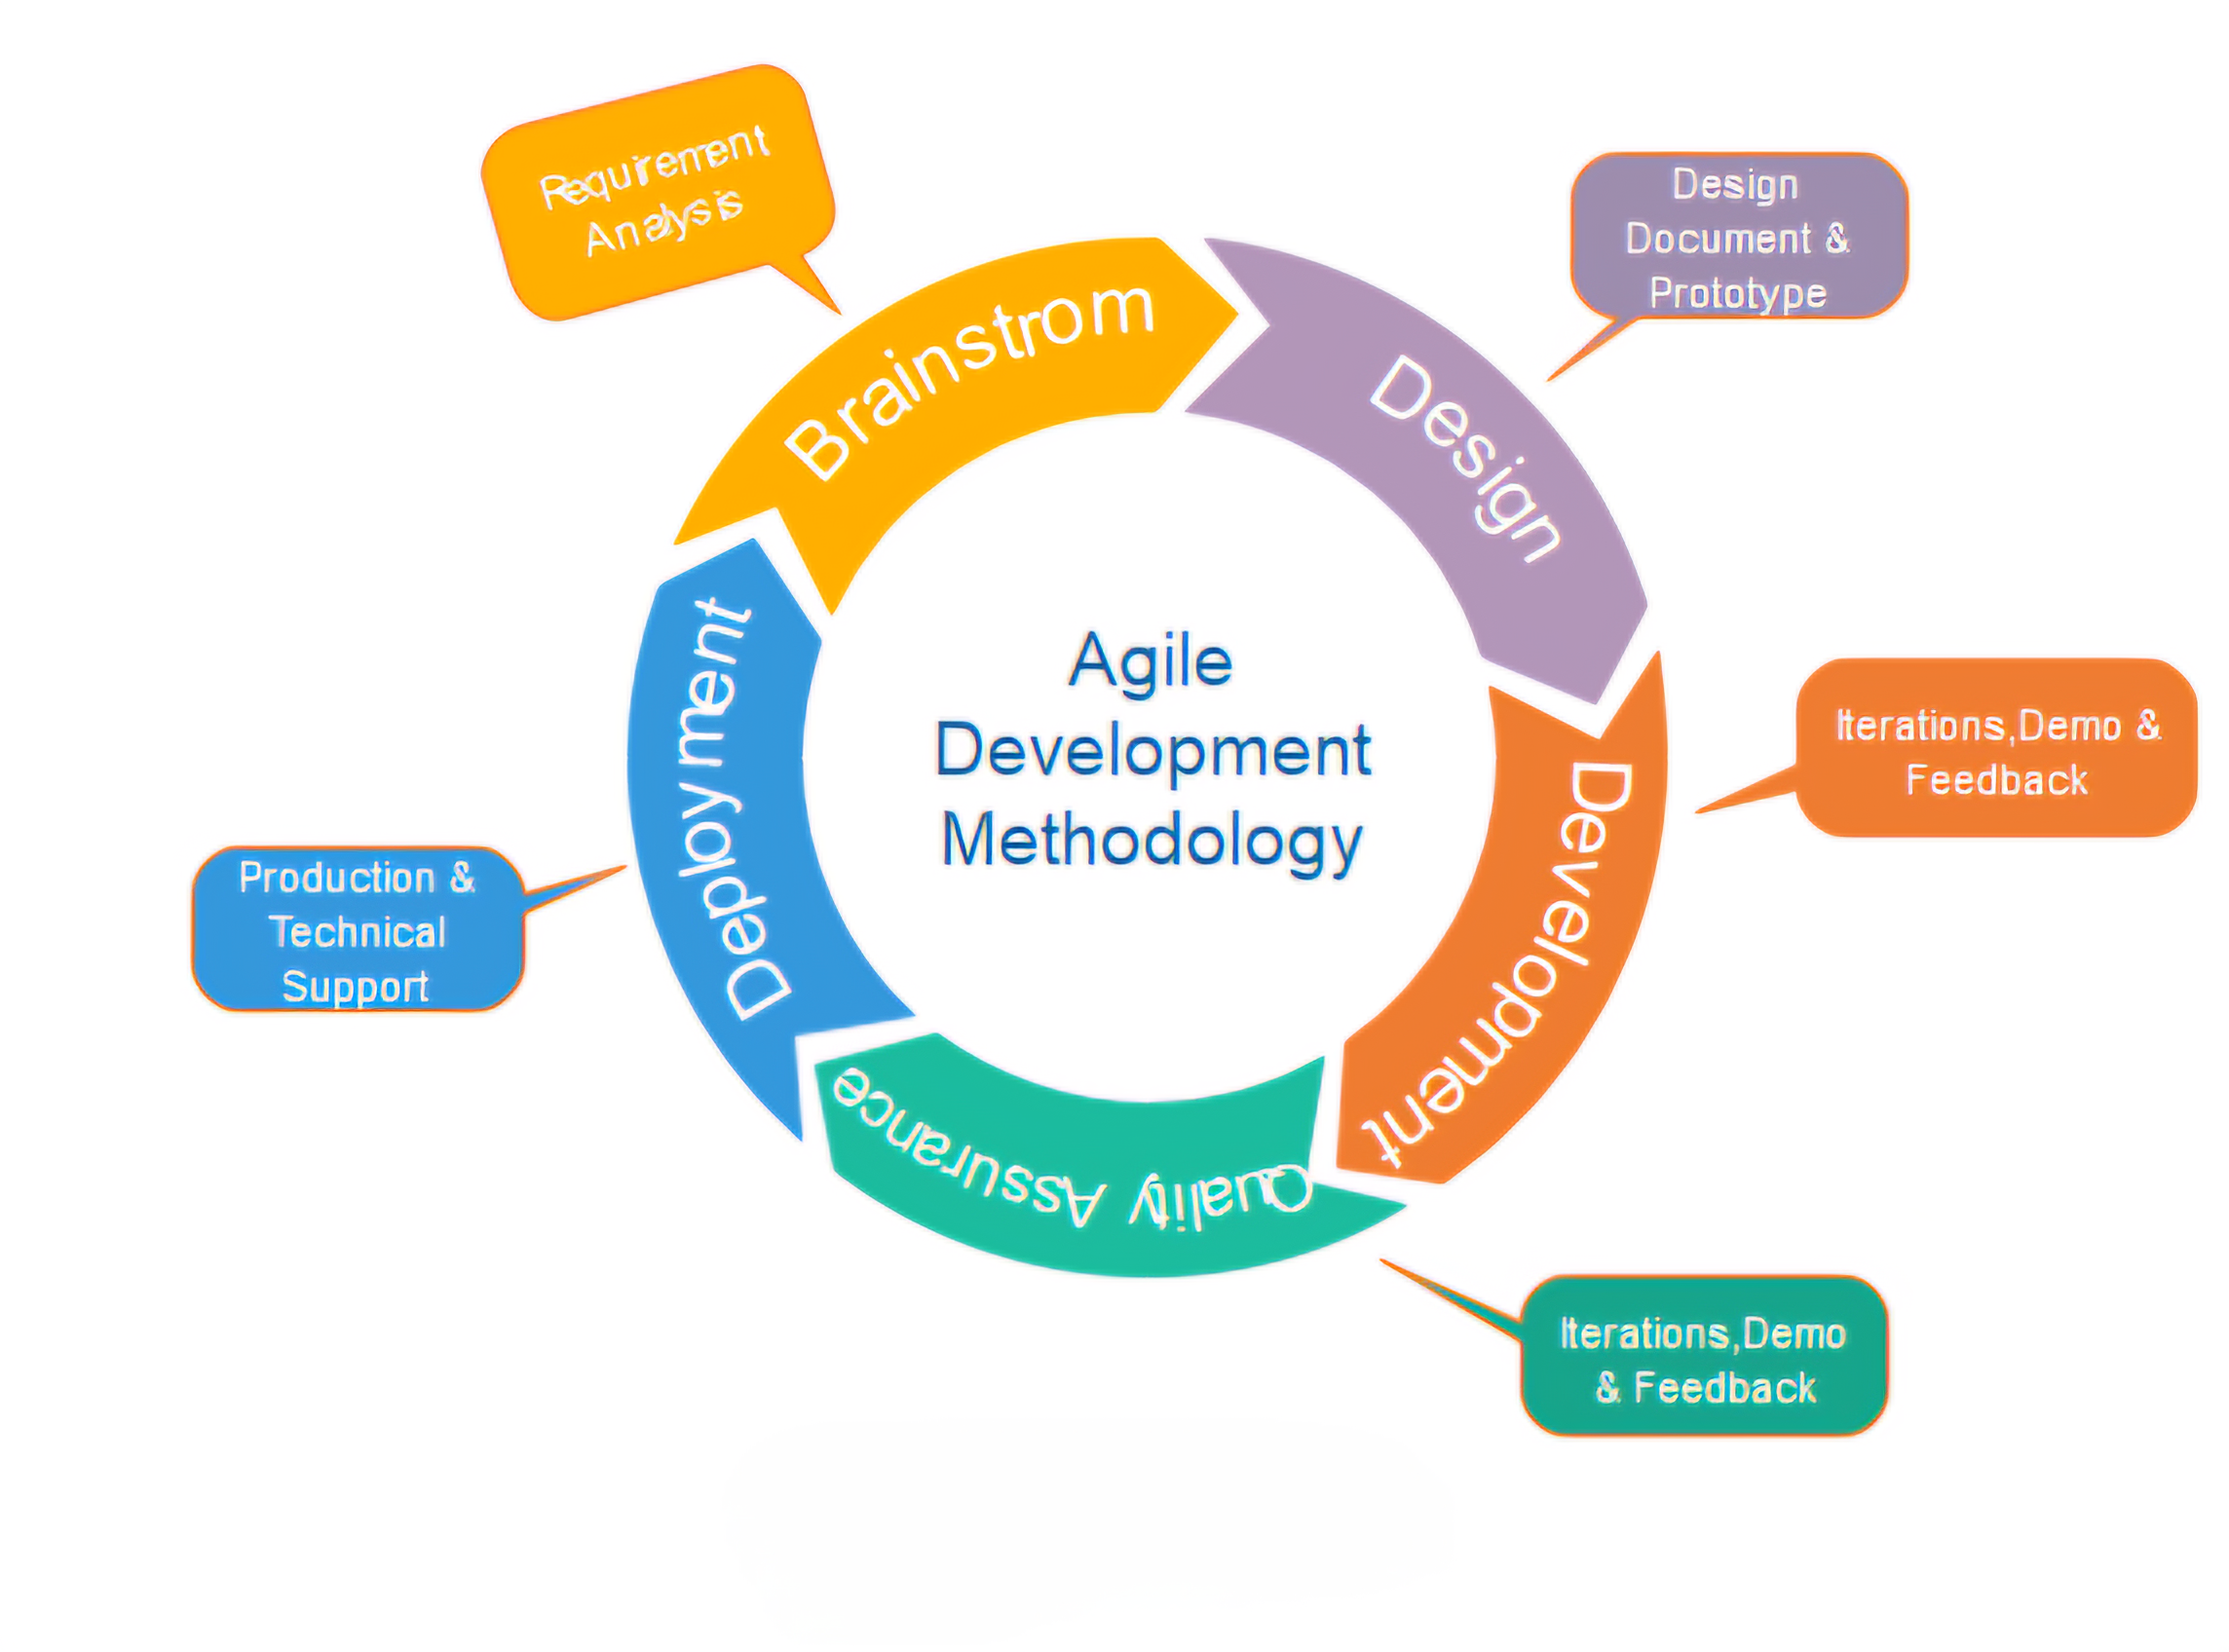
\includegraphics[scale=0.1]{img/agilemodel.png}
        \caption{Agile Development Model}
        \label{fig:agilemodel}
    \end{figure}
\subsection{Agile Sprints}

\subsubsection{Sprint 1: Project Definition and Dataset Exploration}
\textbf{Duration:} Initial Phase\\
\textbf{Goal:} Define the facial inpainting problem and identify suitable datasets for training and evaluation.

\textbf{Key Activities:}
\begin{itemize}
    \item Reviewed existing facial inpainting and image restoration methods.
    \item Explored publicly available face datasets suitable for training and evaluation.
    \item Identified the need to preserve facial structure, texture, and identity during reconstruction.
    \item Defined the main evaluation criteria, including image quality and identity preservation.
\end{itemize}

\textbf{Outcomes:}
\begin{itemize}
    \item Facial inpainting problem and project objectives were clearly defined.
    \item Suitable datasets and evaluation metrics were identified.
    \item Initial system requirements were established.
\end{itemize}


\subsubsection{Sprint 2: Dataset Preparation and Mask Generation}
\textbf{Duration:} Development Phase\\
\textbf{Goal:} Prepare the facial image dataset and generate masked training samples for different facial regions.

\textbf{Key Activities:}
\begin{itemize}
    \item Collected and prepared face images for model training and evaluation.
    \item Generated masks for important facial regions such as the eyes, nose, mouth, and eyebrows.
    \item Applied facial alignment and image resizing to obtain consistent input dimensions.
    \item Prepared masked and corresponding ground-truth image pairs for training.
\end{itemize}

\textbf{Outcomes:}
\begin{itemize}
    \item Training and evaluation data were prepared successfully.
    \item Region-specific facial masks were generated.
    \item The dataset was ready for LGNet training.
\end{itemize}


\subsubsection{Sprint 3: LGNet Architecture and Training Pipeline}
\textbf{Duration:} Development Phase\\
\textbf{Goal:} Design and implement the LGNet-based facial inpainting pipeline.

\textbf{Key Activities:}
\begin{itemize}
    \item Designed the local and global context modules for facial feature reconstruction.
    \item Integrated facial masks and landmark information into the model input.
    \item Implemented the multi-objective loss combining L1, perceptual, style, identity, and landmark losses.
    \item Configured the PyTorch training pipeline with mixed-precision training.
\end{itemize}

\textbf{Outcomes:}
\begin{itemize}
    \item LGNet training architecture was implemented.
    \item The complete training pipeline was successfully configured.
    \item Initial training runs confirmed that the model could reconstruct masked facial regions.
\end{itemize}


\subsubsection{Sprint 4: Model Training and Optimization}
\textbf{Duration:} Training Phase\\
\textbf{Goal:} Train LGNet and improve reconstruction quality while maintaining facial identity.

\textbf{Key Activities:}
\begin{itemize}
    \item Trained the model using PyTorch automatic mixed precision across multiple epochs.
    \item Monitored training and validation losses to evaluate convergence.
    \item Adjusted the training configuration based on observed model performance.
    \item Saved model checkpoints and selected the best-performing checkpoint for evaluation.
\end{itemize}

\textbf{Outcomes:}
\begin{itemize}
    \item Training loss decreased consistently throughout training.
    \item The model reached stable convergence without significant overfitting.
    \item The fifth-epoch checkpoint was selected as the final model checkpoint.
\end{itemize}


\subsubsection{Sprint 5: Boundary Blending and Identity Preservation}
\textbf{Duration:} Refinement Phase\\
\textbf{Goal:} Improve the visual quality of reconstructed regions and preserve the identity of the input face.

\textbf{Key Activities:}
\begin{itemize}
    \item Implemented alpha feathering to reduce visible boundaries around reconstructed regions.
    \item Applied Poisson blending to improve colour and illumination consistency.
    \item Used facial identity embeddings to evaluate identity preservation.
    \item Verified facial landmark consistency between reconstructed and original images.
\end{itemize}

\textbf{Outcomes:}
\begin{itemize}
    \item Boundary artifacts were reduced after post-processing.
    \item Reconstructed regions achieved better visual and structural consistency.
    \item Identity preservation was incorporated into the final evaluation process.
\end{itemize}


\subsubsection{Sprint 6: Evaluation and Comparative Analysis}
\textbf{Duration:} Final Phase\\
\textbf{Goal:} Evaluate the final model and compare its performance with the LaMa baseline.

\textbf{Key Activities:}
\begin{itemize}
    \item Evaluated the final model on the held-out test samples.
    \item Computed PSNR, SSIM, LPIPS, RMSE$_{\log}$, FID, and ArcFace identity scores.
    \item Analysed performance separately for different facial regions.
    \item Compared LGNet results with the LaMa baseline using the stored evaluation metrics.
\end{itemize}

\textbf{Outcomes:}
\begin{itemize}
    \item Final quantitative results were obtained for the proposed model.
    \item LGNet showed strong reconstruction quality and identity preservation.
    \item The final system and evaluation results were prepared for demonstration and reporting.
\end{itemize}

% \newpage
\section{Model Deployment}

This section describes the deployment of the MorphAI system, including the
frontend interface, backend services, trained LGNet model, and the complete
inference pipeline.

\subsection{Frontend Development}

The frontend was developed using React to provide a simple interface for
uploading a facial image and selecting the region to be reconstructed. The
main components include:

\begin{itemize}
    \item Facial image upload with image preview.
    \item Selection of facial regions such as the eyes, nose, eyebrows, and mouth.
    \item Display of the reconstructed facial image.
    \item Before-and-after comparison of the input and generated images.
    \item Status messages for image processing and inference.
\end{itemize}

\noindent Screenshots of the user interface are provided in
Appendices~\ref{app:C1}.

\subsection{Backend Development}

The backend was implemented using Flask to handle image processing and model
inference. Its main responsibilities include:

\begin{itemize}
    \item Receiving the uploaded facial image and selected facial region.
    \item Extracting facial landmarks using the landmark extraction module.
    \item Generating a region-specific mask for the selected facial area.
    \item Creating the facial landmark heatmap required by the model.
    \item Combining the RGB image, mask, and heatmap to form the five-channel
    model input.
    \item Running inference using the trained LGNet generator.
    \item Applying boundary blending to reduce visible seams around the
    reconstructed region.
    \item Returning the final reconstructed image to the frontend.
\end{itemize}

\subsection{Model Integration}

The trained LGNet generator was integrated into the backend for real-time
facial inpainting. The complete inference process follows these steps:

\begin{itemize}
    \item The user uploads an image and selects a facial region.
    \item The backend extracts facial landmarks and generates the corresponding mask.
    \item The RGB image, mask, and landmark heatmap are combined into the
    required five-channel input.
    \item LGNet generates the reconstructed facial region.
    \item Boundary blending is applied to obtain a visually seamless result.
    \item The reconstructed image is returned to the React frontend for display.
\end{itemize}

\noindent The system can additionally use the identity extraction module to
compare the reconstructed face with the original face using facial embeddings.
This helps verify whether the reconstructed result preserves the identity of
the input subject.

\noindent Overall, the deployment integrates the React frontend, Flask backend,
facial preprocessing modules, and LGNet generator into a single end-to-end
facial inpainting system.
    \chapter{CONCLUSION}

\section{Conclusion}

This project successfully developed MorphAI, an identity-preserving facial
inpainting system based on the LGNet architecture. The proposed system
reconstructs masked facial regions while maintaining facial structure, local
textures, and the identity of the input subject. The pipeline combines facial
landmark extraction, region-specific mask generation, landmark heatmaps, and
a five-channel input representation for the LGNet generator.

\noindent The model was trained for five epochs using mixed-precision training on a
dataset containing more than 16,800 facial images. The training loss
decreased consistently, with the fifth epoch selected as the final
convergence checkpoint. Evaluation was performed on 16,800 test samples
across different facial regions and compared with the LaMa baseline.

\noindent The proposed LGNet achieved an overall PSNR of 40.99 dB, SSIM of 0.9928,
ArcFace identity score of 0.9819, RMSE$_{log}$ of 0.0069, and FID of 0.1398.
Compared with LaMa, LGNet provided better structural and identity
preservation, particularly for challenging regions such as the mouth and
nose. These results demonstrate that the proposed approach can effectively
restore facial regions while maintaining the visual characteristics and
identity of the original face.

\section{Limitations}

Despite the promising results, the system has several limitations:

\begin{itemize}
    \item The system is primarily designed for 2D facial image inpainting
    and does not currently reconstruct or represent faces in 3D.
    
    \item The current implementation is not designed as a live or
    real-time video inpainting system and is mainly intended for
    single-image reconstruction.
    
    \item The quality of reconstruction depends on the accuracy of facial
    landmark detection and the generated region mask.
    
    \item Performance may decrease for heavily corrupted regions or
    facial structures with limited surrounding visual information.
    
    \item The model requires GPU resources for efficient inference and
    training, which may limit deployment on low-resource devices.
    
    \item Although ArcFace similarity is used to evaluate identity
    preservation, the identity score does not guarantee perfect
    preservation in every reconstructed image.
\end{itemize}

\section{Future Works}

Based on the findings of this project, several improvements can be explored
in future work:

\begin{itemize}
    \item \textbf{3D Facial Reconstruction:} Extend MorphAI from 2D image
    inpainting to 3D facial reconstruction to model facial geometry and
    provide more realistic results from different viewpoints.
    
    \item \textbf{Real-Time Video Inpainting:} Extend the system to process
    video streams and reconstruct masked facial regions continuously while
    maintaining temporal consistency between frames.
    
    \item \textbf{Dataset Expansion:} Train the model on larger and more
    diverse facial datasets containing different poses, lighting
    conditions, expressions, and degrees of facial occlusion.
    
    \item \textbf{Improved Identity Preservation:} Explore stronger
    identity-aware objectives and modern face-recognition embeddings to
    further improve preservation of facial identity.
    
    \item \textbf{Advanced Generative Models:} Investigate diffusion-based
    and other modern generative architectures to improve reconstruction
    quality for complex facial regions.
    
    \item \textbf{Mobile and Edge Deployment:} Optimize the model through
    techniques such as quantization, pruning, or knowledge distillation
    to enable efficient deployment on resource-constrained devices.
    
    \item \textbf{Interactive Reconstruction:} Develop a more flexible
    interface that allows users to select, adjust, and preview different
    facial regions before generating the final reconstruction.
\end{itemize}

    % ── References ────────────────────────────────────────────────────────────
    \newpage
    \nocite{xu2024diffuse,
        chandaliya2022plasticgan,
        xu2022transeditor,
        tzaban2022stitch,
        bini2025facial,
        chen2024deepface,
        fang2022acmt,
        sun2021maskaware
        }
    \renewcommand{\bibname}{REFERENCES}
    \bibliographystyle{IEEEtran}
    \bibliography{reference}
    \addcontentsline{toc}{chapter}{REFERENCES}

    % ── Appendix ──────────────────────────────────────────────────────────────
    \clearpage
    \appendix
    % ================= Appendix A =================
\chapter{Raw Dataset}
\label{app:A.1}
 \label{fig:samplerawdatas}
\begin{figure}[H]
    \centering
    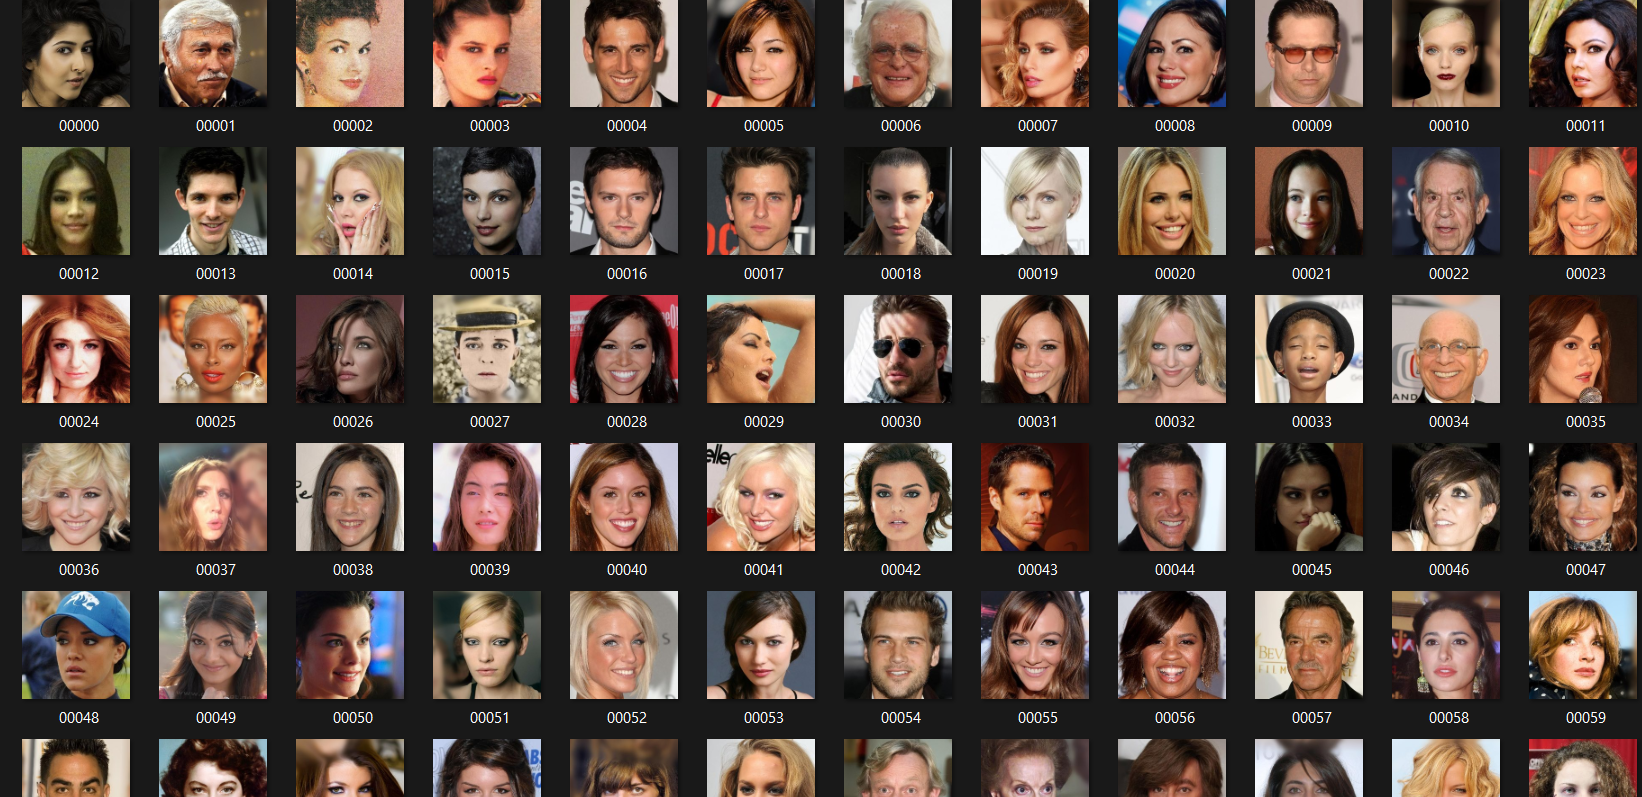
\includegraphics[width=0.75\textwidth]{img/raw_dataset.png}
    \caption{Sample raw dataset}
   
\end{figure}



% ================= Appendix B =================
\chapter{Data Processed}
\label{app:B1}

\section{Data1}
\begin{figure}[H]
    \centering
    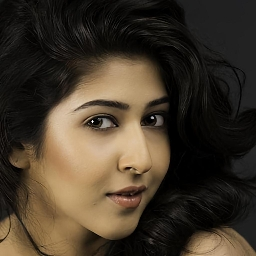
\includegraphics[width=0.5\textwidth]{img/d1.jpeg}
    \caption{Main interface}
\end{figure}

\section{Data1 Landmark}
\begin{figure}[H]
    \centering
    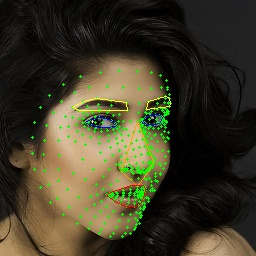
\includegraphics[width=0.5\textwidth]{img/d2.jpeg}
    \caption{Input Image}
\end{figure}

\section{Semantic Masks}

\begin{figure}[H]
\centering

% Row 1
\begin{minipage}{0.48\textwidth}
    \centering
    
\includegraphics[width=0.65\linewidth]{img/2/00000_semantic_left_eye.png}
    \caption{Semantic mask for the left eye region}
    \label{fig:semantic_left_eye}
\end{minipage}
\hfill
\begin{minipage}{0.48\textwidth}
    \centering
    
\includegraphics[width=0.65\linewidth]{img/2/00000_semantic_left_eyebrow.png}
    \caption{Semantic mask for the left eyebrow region}
    \label{fig:semantic_left_eyebrow}
\end{minipage}

\vspace{0.3cm}

% Row 2
\begin{minipage}{0.48\textwidth}
    \centering
    
\includegraphics[width=0.65\linewidth]{img/2/00000_semantic_mouth.png}
    \caption{Semantic mask for the mouth region}
    \label{fig:semantic_mouth}
\end{minipage}
\hfill
\begin{minipage}{0.48\textwidth}
    \centering
    
\includegraphics[width=0.65\linewidth]{img/2/00000_semantic_nose.png}
    \caption{Semantic mask for the nose region}
    \label{fig:semantic_nose}
\end{minipage}

\vspace{0.3cm}

% Row 3
\begin{minipage}{0.48\textwidth}
    \centering
    
\includegraphics[width=0.65\linewidth]{img/2/00000_semantic_right_eye.png}
    \caption{Semantic mask for the right eye region}
    \label{fig:semantic_right_eye}
\end{minipage}
\hfill
\begin{minipage}{0.48\textwidth}
    \centering
    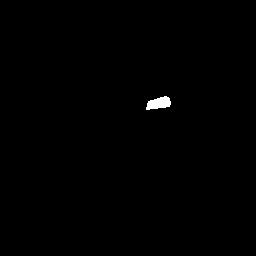
\includegraphics[width=0.65\linewidth]{img/2/00000_semantic_right_eyebrow.png}
    \caption{Semantic mask for the right eyebrow region}
    \label{fig:semantic_right_eyebrow}
\end{minipage}

\end{figure}

\clearpage

\section{Heatmaps}

\begin{figure}[H]
\centering

% Row 1
\begin{minipage}{0.48\textwidth}
    \centering
    
\includegraphics[width=0.65\linewidth]{img/1/1_00000_semantic_left_eye.png}
    \caption{Landmark heatmap for the left eye region}
    \label{fig:heatmap_left_eye}
\end{minipage}
\hfill
\begin{minipage}{0.48\textwidth}
    \centering
    
\includegraphics[width=0.65\linewidth]{img/1/1_00000_semantic_left_eyebrow.png}
    \caption{Landmark heatmap for the left eyebrow region}
    \label{fig:heatmap_left_eyebrow}
\end{minipage}

\vspace{0.3cm}

% Row 2
\begin{minipage}{0.48\textwidth}
    \centering
    
\includegraphics[width=0.65\linewidth]{img/1/1_00000_semantic_mouth.png}
    \caption{Landmark heatmap for the mouth region}
    \label{fig:heatmap_mouth}
\end{minipage}
\hfill
\begin{minipage}{0.48\textwidth}
    \centering
    
\includegraphics[width=0.65\linewidth]{img/1/1_00000_semantic_nose.png}
    \caption{Landmark heatmap for the nose region}
    \label{fig:heatmap_nose}
\end{minipage}

\vspace{0.3cm}

% Row 3
\begin{minipage}{0.48\textwidth}
    \centering
    
\includegraphics[width=0.65\linewidth]{img/1/1_00000_semantic_right_eye.png}
    \caption{Landmark heatmap for the right eye region}
    \label{fig:heatmap_right_eye}
\end{minipage}
\hfill
\begin{minipage}{0.48\textwidth}
    \centering
    
\includegraphics[width=0.65\linewidth]{img/1/1_00000_semantic_right_eyebrow.png}
    \caption{Landmark heatmap for the right eyebrow region}
    \label{fig:heatmap_right_eyebrow}
\end{minipage}

\end{figure}


% ================= Appendix C =================
\chapter{Image Pre-processing Pipeline Details}
\label{app:preprocessing}
\section{Original Input (256*256)}
\label{app:C1}
\begin{figure}[H]
    \centering
    
\includegraphics[width=0.5\textwidth]{img/b1.jpeg}
    \caption{Original Input (256*256)}
\end{figure}

\section{Landmarks Detection}
\label{app:C2}
\begin{figure}[H]
    \centering
    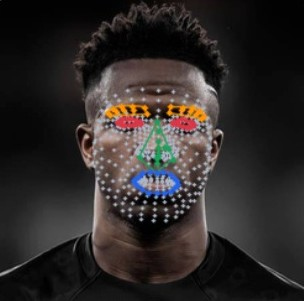
\includegraphics[width=0.5\textwidth]{img/b2.jpeg}
    \caption{Landmarks Detection}
\end{figure}

\section{Masked Input}
\label{app:C3}
\begin{figure}[H]
    \centering
    
\includegraphics[width=0.5\textwidth]{img/b3.jpeg}
    \caption{Masked Input}
\end{figure}

\section{Binary Mask}
\label{app:C4}
\begin{figure}[H]
    \centering
    
\includegraphics[width=0.5\textwidth]{img/b4.jpeg}
    \caption{Binary Mask}
\end{figure}

\section{Landmark Heatmap}
\label{app:C5}
\begin{figure}[H]
    \centering
    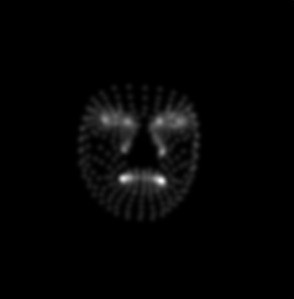
\includegraphics[width=0.5\textwidth]{img/b5.jpeg}
    \caption{Landmark Heatmap}
\end{figure}

\section{Raw Generator Output}
\label{app:C6}
\begin{figure}[H]
    \centering
    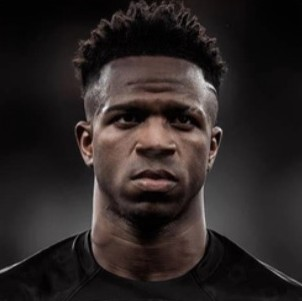
\includegraphics[width=0.5\textwidth]{img/b6.jpeg}
    \caption{Raw Generator Output}
\end{figure}

\section{Reconstructed Output}
\label{app:C7}
\begin{figure}[H]
    \centering
    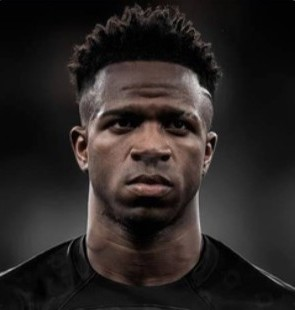
\includegraphics[width=0.5\textwidth]{img/b7.jpeg}
    \caption{Reconstructed Output}
\end{figure}


% ================= Appendix D =================
\chapter{User Interface Screenshots}
\label{app:D1}

\section{Main Interface}
\begin{figure}[H]
    \centering
    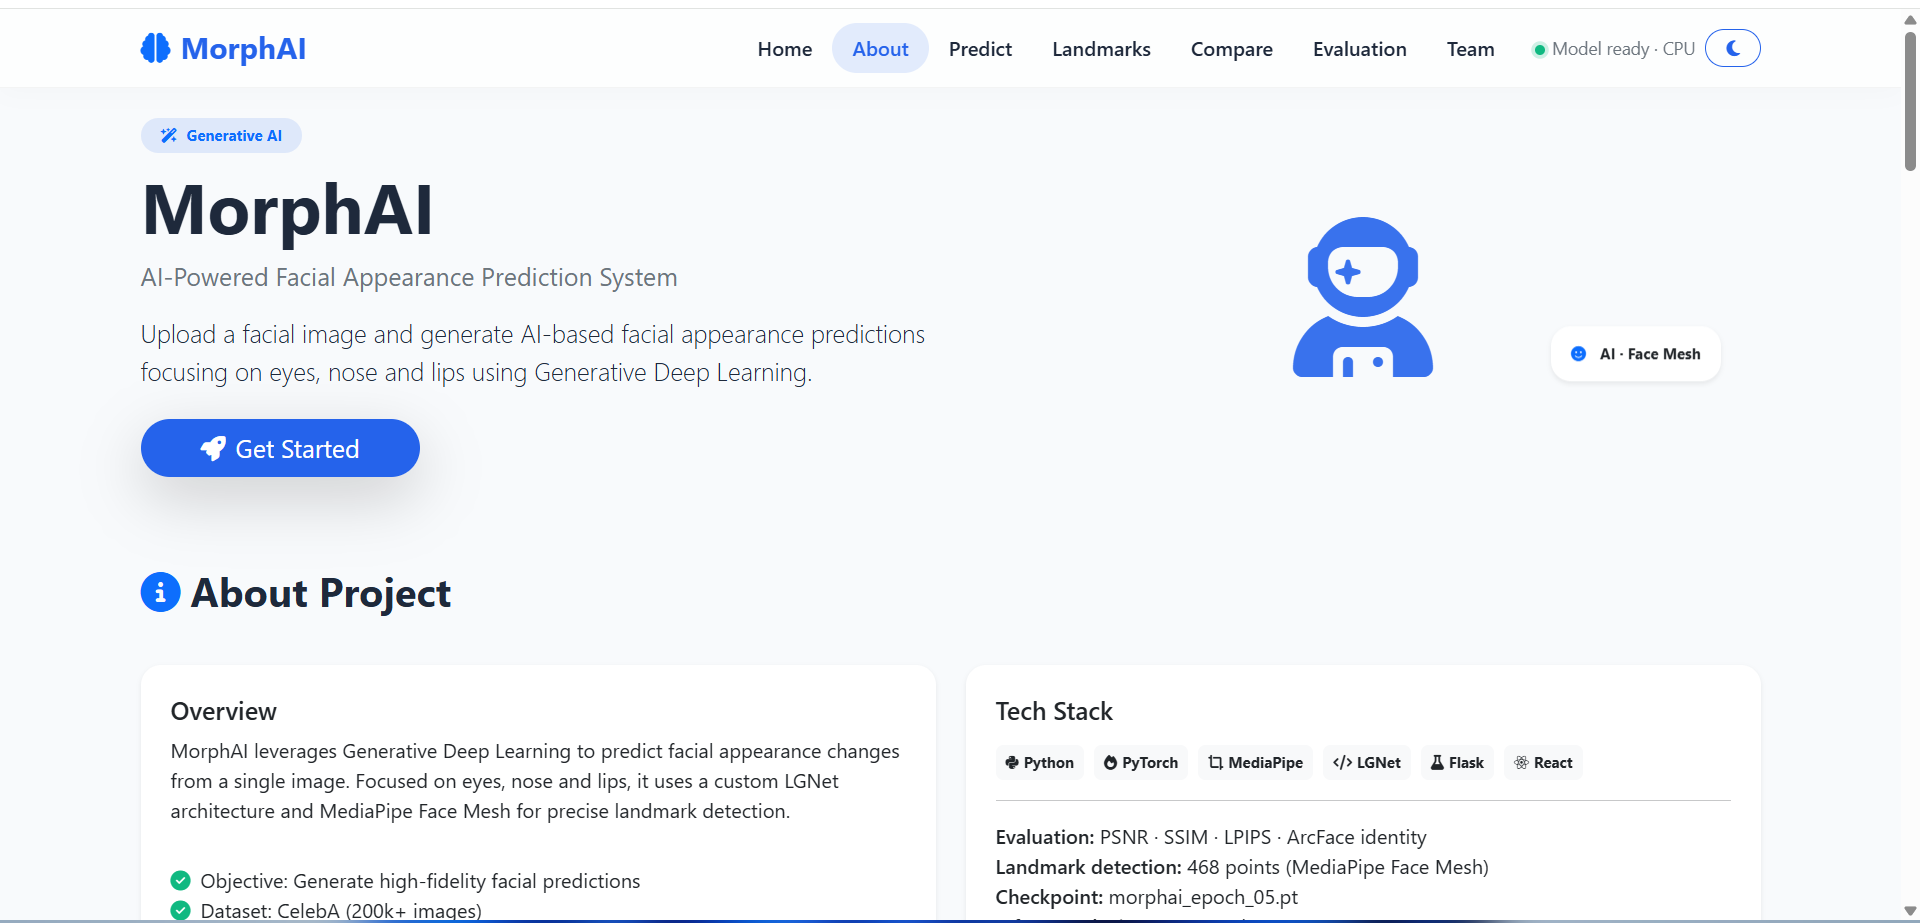
\includegraphics[width=0.72\textwidth]{img/UI.png}
    \caption{Main interface}
\end{figure}

\section{Input Image}
\begin{figure}[H]
    \centering
    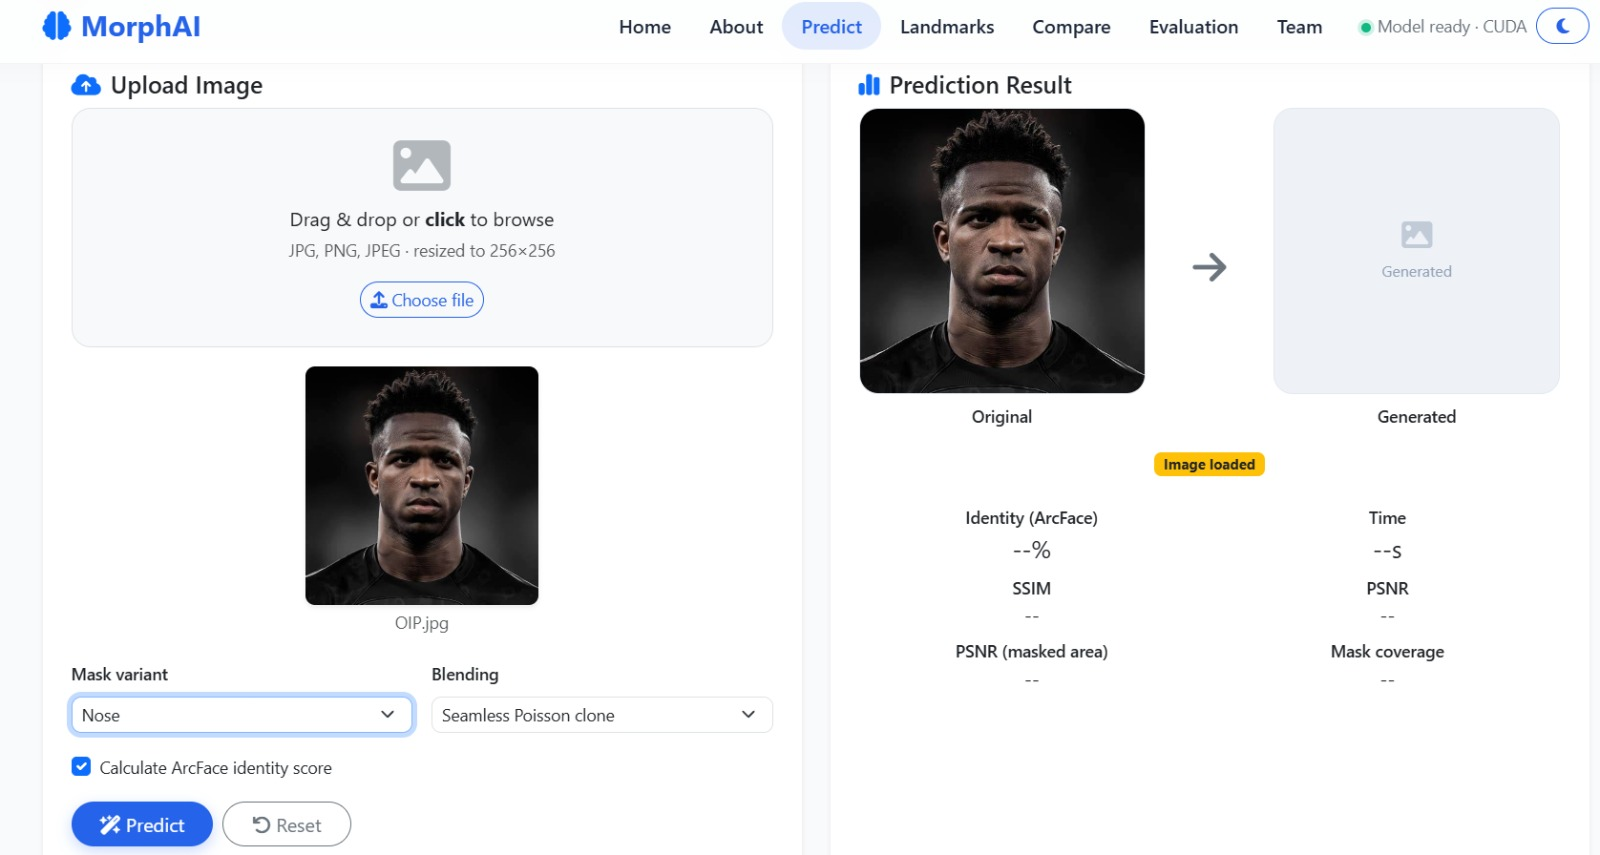
\includegraphics[width=0.75\textwidth]{img/c1.jpeg}
    \caption{Input Image}
\end{figure}

\section{Facial Landmark}
\begin{figure}[H]
    \centering
    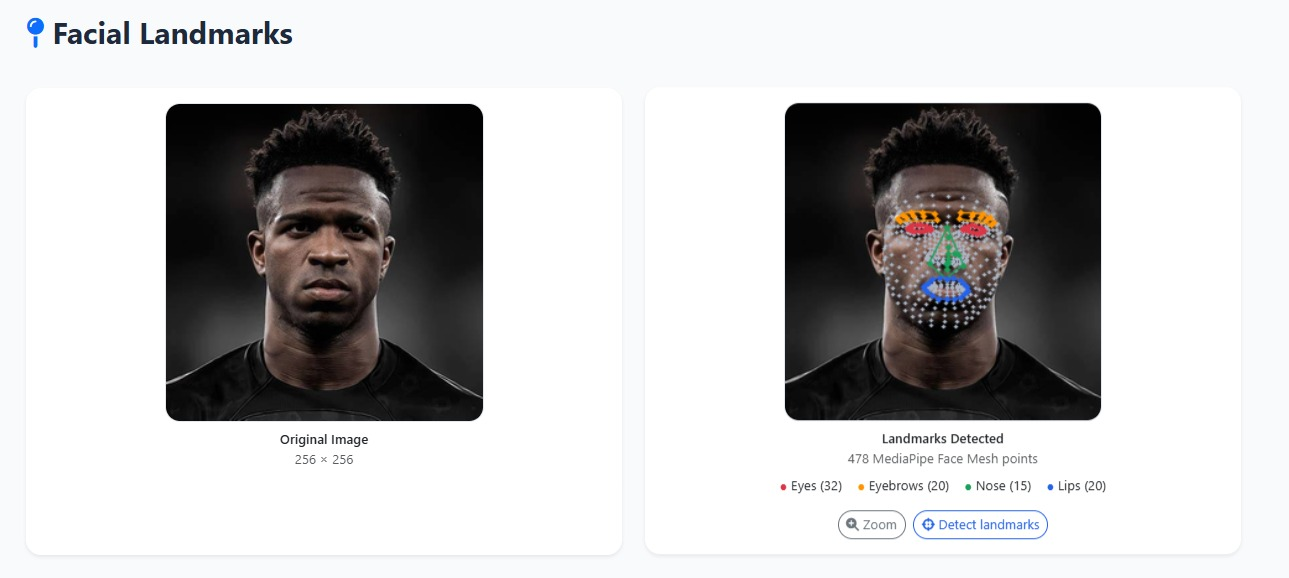
\includegraphics[width=0.75\textwidth]{img/c2.jpeg}
    \caption{Facial Landmark}
\end{figure}

\section{Inference Pipeline}
\begin{figure}[H]
    \centering
    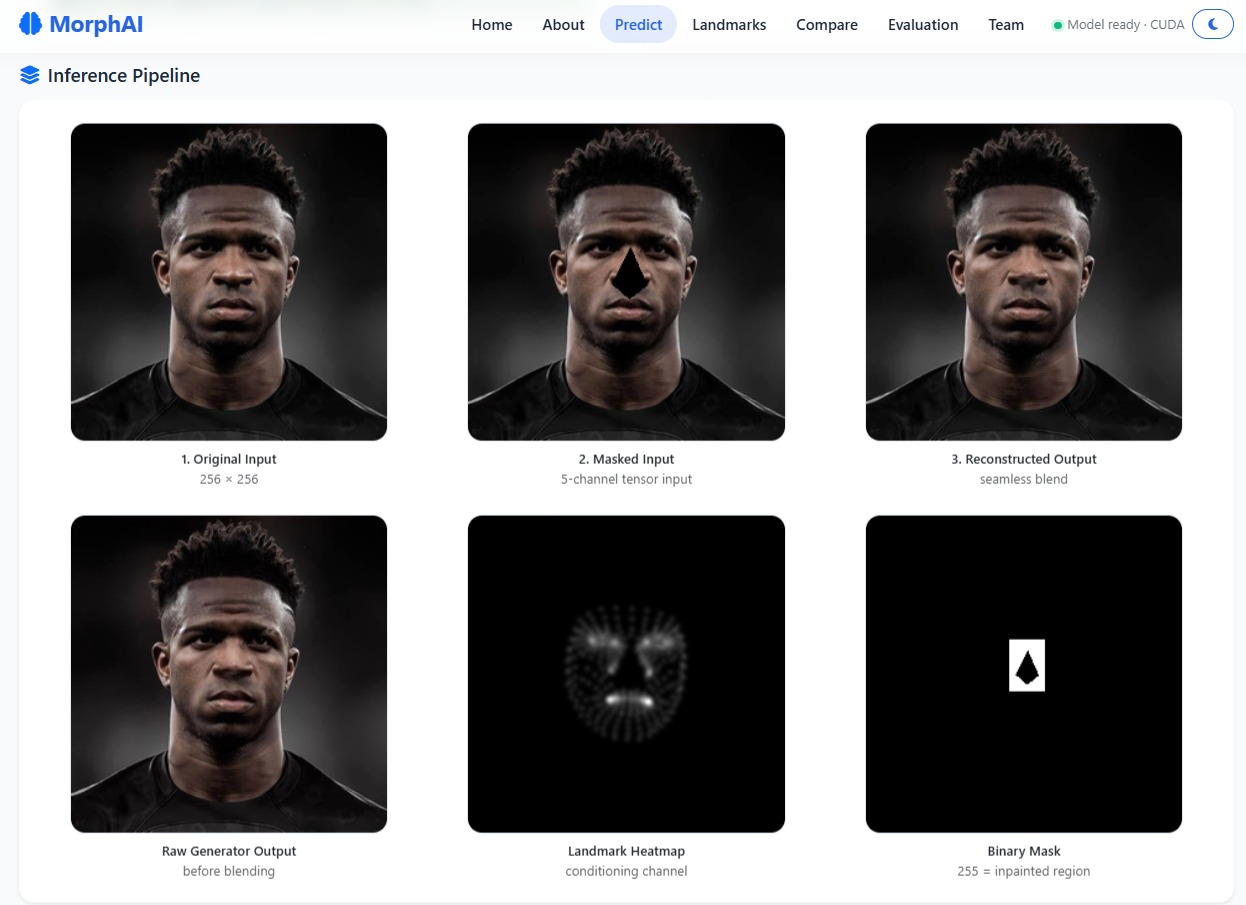
\includegraphics[width=0.75\textwidth]{img/c3.jpeg}
    \caption{Inference Pipeline}
\end{figure}

\section{Predicted Output}
\begin{figure}[H]
    \centering
    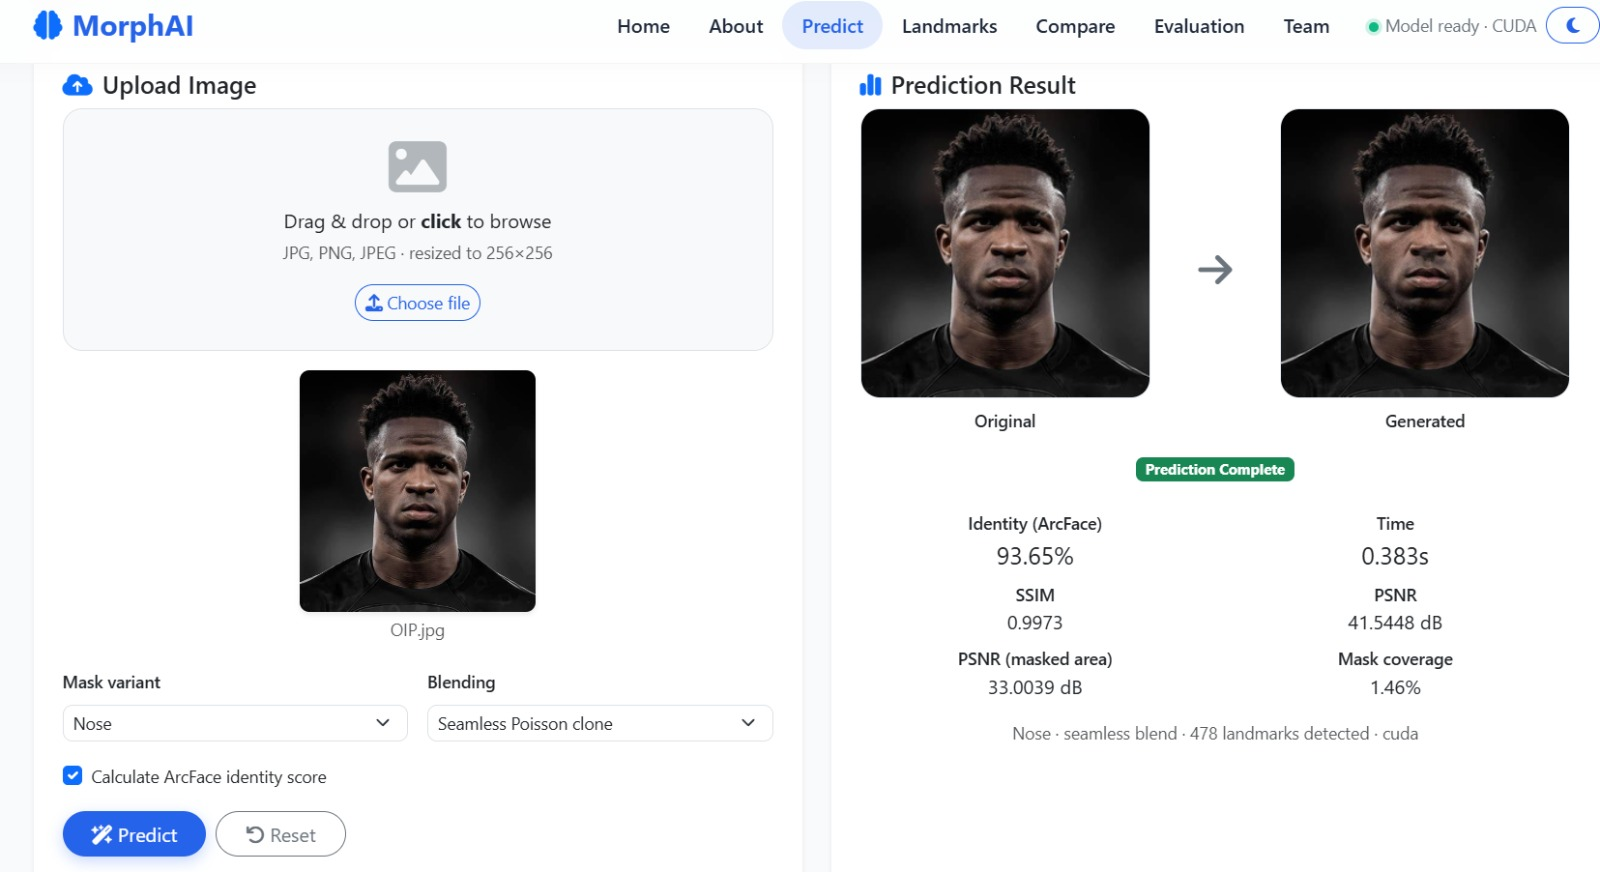
\includegraphics[width=0.75\textwidth]{img/c4.jpeg}
    \caption{Predicted Output}
\end{figure}

\end{document}